% Template file for a standard thesis
\documentclass[11pt]{isuthesis}\usepackage[]{graphicx}\usepackage[]{color}
%% maxwidth is the original width if it is less than linewidth
%% otherwise use linewidth (to make sure the graphics do not exceed the margin)
\makeatletter
\def\maxwidth{ %
  \ifdim\Gin@nat@width>\linewidth
    \linewidth
  \else
    \Gin@nat@width
  \fi
}
\makeatother

\definecolor{fgcolor}{rgb}{0.345, 0.345, 0.345}
\newcommand{\hlnum}[1]{\textcolor[rgb]{0.686,0.059,0.569}{#1}}%
\newcommand{\hlstr}[1]{\textcolor[rgb]{0.192,0.494,0.8}{#1}}%
\newcommand{\hlcom}[1]{\textcolor[rgb]{0.678,0.584,0.686}{\textit{#1}}}%
\newcommand{\hlopt}[1]{\textcolor[rgb]{0,0,0}{#1}}%
\newcommand{\hlstd}[1]{\textcolor[rgb]{0.345,0.345,0.345}{#1}}%
\newcommand{\hlkwa}[1]{\textcolor[rgb]{0.161,0.373,0.58}{\textbf{#1}}}%
\newcommand{\hlkwb}[1]{\textcolor[rgb]{0.69,0.353,0.396}{#1}}%
\newcommand{\hlkwc}[1]{\textcolor[rgb]{0.333,0.667,0.333}{#1}}%
\newcommand{\hlkwd}[1]{\textcolor[rgb]{0.737,0.353,0.396}{\textbf{#1}}}%

\usepackage{framed}
\makeatletter
\newenvironment{kframe}{%
 \def\at@end@of@kframe{}%
 \ifinner\ifhmode%
  \def\at@end@of@kframe{\end{minipage}}%
  \begin{minipage}{\columnwidth}%
 \fi\fi%
 \def\FrameCommand##1{\hskip\@totalleftmargin \hskip-\fboxsep
 \colorbox{shadecolor}{##1}\hskip-\fboxsep
     % There is no \\@totalrightmargin, so:
     \hskip-\linewidth \hskip-\@totalleftmargin \hskip\columnwidth}%
 \MakeFramed {\advance\hsize-\width
   \@totalleftmargin\z@ \linewidth\hsize
   \@setminipage}}%
 {\par\unskip\endMakeFramed%
 \at@end@of@kframe}
\makeatother

\definecolor{shadecolor}{rgb}{.97, .97, .97}
\definecolor{messagecolor}{rgb}{0, 0, 0}
\definecolor{warningcolor}{rgb}{1, 0, 1}
\definecolor{errorcolor}{rgb}{1, 0, 0}
\newenvironment{knitrout}{}{} % an empty environment to be redefined in TeX

\usepackage{alltt}
%---------------------------------------------------
\usepackage{color}
\usepackage[dvipsnames,svgnames]{xcolor}
\usepackage{wrapfig,float}
\usepackage{caption}
\usepackage{subcaption}
\usepackage{graphicx}
\usepackage{amssymb}
\usepackage{amsmath}
\usepackage{url}
\usepackage{ulem}
\usepackage[section]{placeins}
\usepackage{sidecap}
\usepackage{multirow}
\usepackage{bbm}
\usepackage[colorinlistoftodos]{todonotes}
%---------------------------------------------------

% Standard, old-style thesis
\usepackage{isutraditional}   \chaptertitle
% Old-style, thesis numbering down to subsubsection
\alternate
\usepackage{rotating}
% Bibliography without numbers or labels
\usepackage{natbib}
\bibliographystyle{apa}
%\includeonly{titletoc,chapter1}
%Optional Package to add PDF bookmarks and hypertext links
\usepackage[pdftex,hypertexnames=false,linktocpage=true]{hyperref}
\hypersetup{colorlinks=true,linkcolor=blue,anchorcolor=blue,citecolor=blue,filecolor=blue,urlcolor=blue,bookmarksnumbered=true,pdfview=FitB}

\newcommand{\done}[2][inline]{\todo[color=SpringGreen, #1]{#2}}  % for todos that have been seen and dealt with
\newcommand{\meh}[2][inline]{\todo[color=White, #1]{#2}}   % for todos that may no longer be relevant 
\newcommand{\comment}[2][inline]{\todo[color=SkyBlue, #1]{#2}} % for comments that may not be "to-do"s
\newcommand{\mcomment}[1]{\todo[color=SkyBlue]{#1}} % for margin comments

\newcommand{\newtext}[1]{\todo[inline, color=White]{ \color{OliveGreen}{#1}}} % new text - not necessarily something to be done

\newcommand{\move}[1]{\todo[inline, color=Lime]{#1}} % new to do item

%---------------------------------------------------


\IfFileExists{upquote.sty}{\usepackage{upquote}}{}
\begin{document}
\DeclareGraphicsExtensions{.jpg,.pdf,.mps,.png}
%-------------------------------------------------------------------------------
% Template Titlepage File
\title{This is the title of a thesis
submitted to Iowa State University\\
Note that only the first letter of
the first word and proper names
are capitalized}
\author{Wilbur Terrance Johnson}
\degree{MASTER OF SCIENCE}
\major{Human Development and Family Studies (Marriage and Family Therapy)}
\level{master's}
\mprof{Susan D. Ross}
\members{Mary Jones \\ Bjork Petersen}
\notice
% Add these additional lines for a Doctoral Dissertation
%\degree{DOCTOR OF PHILOSOPHY}
%\level{doctoral}
%\format{dissertation}
%\committee{4}
%\members{Mary Jones \\ Bjork Petersen \\ Sam Anders \\ Harold Jones}
% Add these additional lines for a Creative Component
% - also comment out the \maketitle command
%\format{Creative Component}
%\submit{the graduate faculty}
\maketitle

%-------------------------------------------------------------------------------
% Optional thesis dedication
% \chapter*{DEDICATION}

I would like to dedicate this thesis to my wife Glenda and
to my daughter Alice without whose support I would not have
been able to complete this work.
I would also like to thank my friends and family for their loving guidance and
financial assistance during the writing of this work.


%-------------------------------------------------------------------------------
% Table of Contents, List of Tables and List of Figures
\pdfbookmark[1]{TABLE OF CONTENTS}{table}
\tableofcontents
\addtocontents{toc}{\def\protect\@chapapp{}} \cleardoublepage \phantomsection
\addcontentsline{toc}{chapter}{LIST OF TABLES}
\listoftables
\cleardoublepage \phantomsection \addcontentsline{toc}{chapter}{LIST OF FIGURES}
\listoffigures
% Comment out the next line if NOT using chaptertitle
\addtocontents{toc}{\def\protect\@chapapp{CHAPTER\ }}
%-------------------------------------------------------------------------------
%Optional Acknowledgements
% \cleardoublepage \phantomsection
% \specialchapt{ACKNOWLEDGEMENTS}

I would like to take this opportunity to express my thanks to those
who helped me with various aspects of conducting research and the writing
of this thesis.
First and foremost, Dr. Susan D. Ross for her guidance, patience and support
throughout this research and the writing of this thesis.
Her insights and words of encouragement have often inspired me and renewed
my hopes for completing my graduate education.
I would also like to thank my committee members for their efforts
and contributions to this work: Dr. August Tanner and
Dr. Lewis Hargrave.
I would additionally like to thank
Dr. Tanner for his guidance throughout the initial stages of my
graduate career and Dr. Hargrave for his inspirational teaching style.

%-------------------------------------------------------------------------------
%Optional thesis abstract
% \cleardoublepage \phantomsection
% \specialchapt{ABSTRACT}

This is the text of my abstract that is part of the thesis itself.
The abstract describes the work in general and the heading and style
match the rest of the document.

%-------------------------------------------------------------------------------
\newpage
\pagenumbering{arabic}
%-------------------------------------------------------------------------------


\graphicspath{{Figure/LitReview/}{Images/LitReview/}}
\renewcommand{\floatpagefraction}{.99}





% Chapter 1 of the Thesis Template File
\chapter{OVERVIEW}

\section{Goals of Statistical Graphics}

\section{The Human Visual System}
Basic overview of structure, to serve as a reference

In order to design graphics for the human perceptual system, we must understand, at a basic level, the makeup of the perceptual system. There are multiple levels of perception that must correctly function in order to perceive visual stimuli successfully, but a somewhat simplistic higher-level analogy would be that we must understand both the hardware and software of the human visual system to create effective graphics.
The ``hardware", in this analogy, consists of the neurons that make up the eyes, optic nerve, and the brain itself. The higher-level functions (object recognition, working memory, etc.) comprise the ``software" component. In addition, much like computer software, there are different programs running simultaneously; these programs may interact with each other, run sequentially, or run in parallel. The following sections provide an overview of the grey-matter (hardware) components of the visual system as well as the higher-level cognitive heuristics (software) that order the raw input and construct our visual environment. 

\subsection{Hardware}
The physiology of perception is complex; what follows is a high-level overview of the physiology of perception, focusing on the areas most important to the perception of statistical graphics. This physiological information is important in understanding the difference between the sensation (i.e. the retinal image) and the perception (the corresponding mental representation), which is an important distinction in understanding how statistical graphics are perceived. 

\paragraph{The Eye}
The eye is a complex apparatus, but for our purposes, the primary component of the eye is the retina, which contains the sensory cells responsible for transforming light waves into electrical information in the form of neural signals. 
These sensory cells are specialized neurons, known as rods and cones, which perceive light intensity (brightness) and wavelength (color), respectively. One section of the retina, known as the fovea, contains only cones; the rest of the retina contains a mixture of rods and cones. Figure \ref{fig:retina} depicts the structure of the eye with a closeup of the retina. 

\begin{figure}
\centering
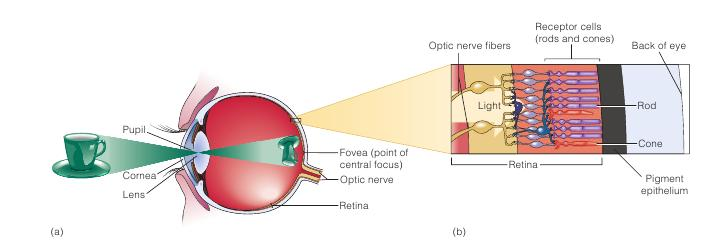
\includegraphics[width=.8\textwidth, keepaspectratio=TRUE]{Figure/LitReview/Retina}
\caption[The human eye, with closeup of receptor cells in the retina]{The human eye, with closeup of receptor cells in the retina (image from \protect\citealt{goldstein}, chap 3.1).} \label{fig:retina}
\end{figure}

\begin{figure}
\centering
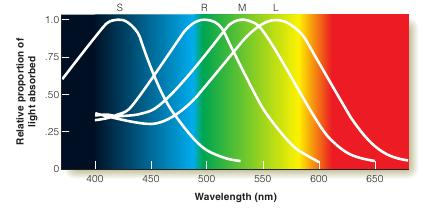
\includegraphics[width=.8\textwidth, keepaspectratio=TRUE]{Figure/LitReview/AbsorptionSpectra}
\caption[Absorption spectra of retinal cells]{Absorption spectra of rods and short, medium, and long wave cones. (image from \protect\citealt{goldstein}, chap 3.3).} \label{fig:ColorRange}
\end{figure}

Figure \ref{fig:ColorRange} shows the responsiveness of rods and each of the three types of cones to wavelengths of light in the visual spectrum. This image suggests that we have relatively good visual discrimination of the yellow-green portion of the color spectrum, but relatively poor discrimination of colors in the red and blue portions of the color spectrum. As a result, rainbow-style color schemes are seldom appropriate for conveying numerical values, because the correspondance between the perceived information and the displayed information is not accurately maintained by the visual system \citep{rainbowcolor}. In addition, if any of the cones are missing or damaged as a result of genetic mutations, color perception is impaired, resulting in a smaller range of distinguishable colors. This set of impairments is known coloquially as color-blindness, and occurs in an estimated 5\% of the population. 

\paragraph{The Brain}
Once light hits the retina and causes a signal in the receptor cells, the information travels along the optic nerve and into the brain. Multiple neighboring rods are connected to the same neuron, where each cone is connected to its' own neuron. The combined wiring of rod cells is responsible for the Hermann grid illusion and the Mach bands seen in Figure \ref{fig:InhibitionIllusions}. Both of these illusions are a product of lateral inhibition, which is a result of the wiring of rod cells in the retina.  The specifics of the wiring of the receptor cells are somewhat complex; a more thorough explanation can be found in \citet{goldstein}, chapter 3.4. 

\begin{figure}
\centering
\begin{subfigure}[b]{.45\textwidth}
  \centering
  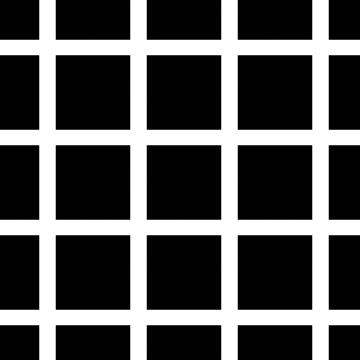
\includegraphics[width=\textwidth]{Figure/LitReview/HermannGrid}
  \caption{\small Hermann Grid Illusion \label{fig:hermanngrid}}
\end{subfigure}\hfill
\begin{subfigure}[b]{.45\textwidth}
  \centering
  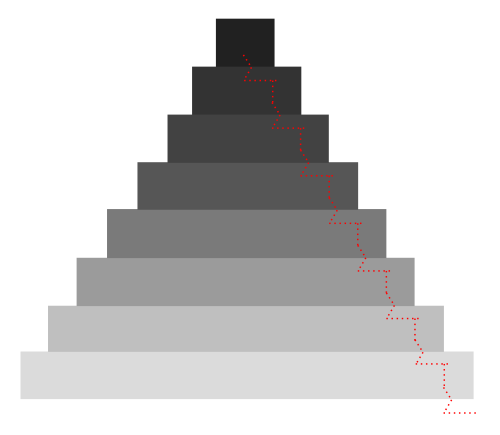
\includegraphics[width=\textwidth]{Figure/LitReview/MachBands}
  \caption{\small Mach Bands. 
  \label{fig:machbands}}
\end{subfigure}
\caption[Inhibition Illusions]{Optical Illusions resulting from lateral inhibition. The Hermann Grid illusion causes dark circles to appear at the intersection of white lines; the Mach bands illusion causes the borders of adjacent rectangles to appear more strongly defined.} \label{fig:InhibitionIllusions}
\end{figure}

Once neural impulses have left the retina through the optic nerve, they travel to the visual cortex by way of several specialized structures within the brain that process lower-level signals. Receptor cells in the visual cortext respond to specific angles, spatial locations, colors, and intensities, and arrays of these special 'feature detector cells' process the information into a form that higher-level processes can utilize. These higher-level processes are what we have previously called 'software': they are not directly related to the physical brain, but they do process information heuristically to produce higher-level reasoning and conclusions. In the next section, we explore some of the higher-level processes responsible for visual perception.

\subsection{Software}\label{Software}
Many of the processes for visual perception run simultaneously; in absence of a temporal ordering, we will start with the more basic tasks of visual perception and proceed towards higher-level processes. We will begin with attention.

\subsubsection{Attention and Perception} \label{AttentionPerception}
In many tasks, it is necessary to pay attention to many different input streams simultaneously; this is particularly true for complex tasks like driving a car. These tasks demand divided attention; the brain must process many different sources of information in parallel. By contrast, most image recognition tasks require selective attention, that is, focusing on specific objects and ignoring everything else. The brain accomplishes this attention through several mechanisms. 

Selective attention is accomplished by focusing the fovea (the area with the highest visual acuity) on the object. For instance, if the object is a page of text, each word will pass through the fovea, producing a focused stream of visual input. This stream of input consists of saccades (jumps between points of focus) and pauses in which the visual information is relayed to the brain. Figure \ref{fig:saccadestext} shows the saccades (lines) and pauses (circles) resulting when someone scans a paragraph of text. These saccades and pauses are utilized in eye-tracking technology to determine which parts of an image the observer is focusing on (and by extension, which information is being encoded by the brain). 

\begin{figure}[h]
\centering
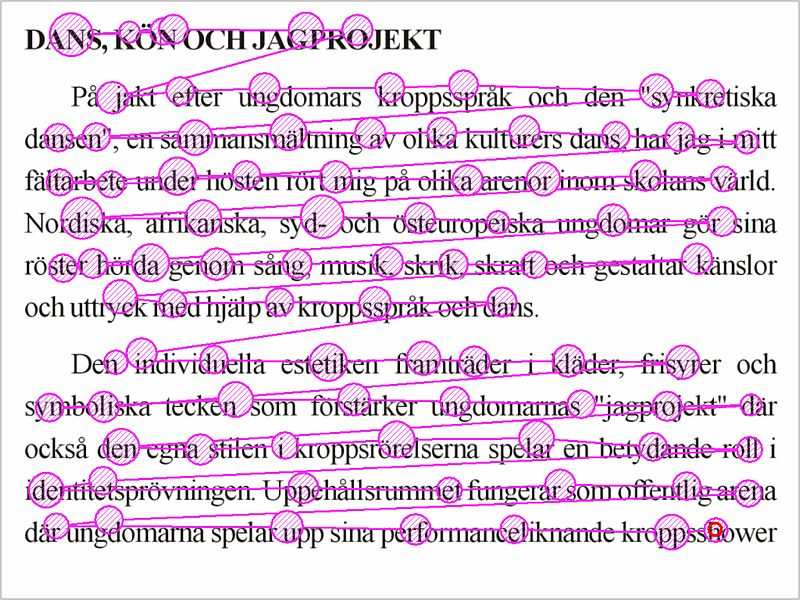
\includegraphics[width=.5\textwidth]{SaccadesText}
\caption[Saccades and Pauses]{A plot of saccades made while reading text. Saccades, shown by the lines, indicate ``jumps", while pauses are shown by circles, with size proportional to the time spent focusing on that area.}\label{fig:saccadestext}
\end{figure}

Selective attention is generally necessary for perception to occur, though there is some information that is encoded automatically. Experiments such as the fairly famous \href{http://www.theinvisiblegorilla.com/videos.html}{"gorilla" film}\footnote{\url{http://www.theinvisiblegorilla.com/videos.html}} demonstrate that even when there is attention focused on a task, information extraneous to that task is not always encoded, that is, even when participants focused on counting the number of passes of the basketball, they did not notice the obvious gorilla walking through the scene. It is important to understand which parts of a visual stimulus are the focus of a given perceptual task, because most of the information encoded by the brain is a result of selective attention. Eye-tracking can be an important tool useful to understand these perceptual processes, but participants are often able to report which parts of a stimulus contributed to their decision as well.

Within the brain, attention is important because it allows different regions of the brain which process color, shape, and position to integrate these perceptions into a multifaceted mental representation of the object \citep{goldstein}. This process, known as binding, is essential to coherently encode a scene into working memory. Feature integration theory \citep{treisman1980feature} suggests that these separate streams of information are initially encoded in the preattentive stage of object perception; focusing on the object triggers the binding of these separate streams into a single coherent stream of information. Many single features, such as color, length, and texture are \emph{preattentive}, because they can be pinpointed in an image without focused attention (and thus can be located faster), but specific combinations of color and shape require attention (because the features must be bound together) and are thus more difficult to search. Preattentive features are generally processed in parallel (that is, the entire scene is processed nearly simultaneously), while features requiring attention are processed serially. Examples of features processed  serially and in parallel are shown in Figure \ref{fig:parallelSerialFeatures}, taken from Chapter 6 of \citet{helander1997handbook}. The importance of preattentive processing to statistical graphics is discussed in Section \ref{LowLevelGraphics}. 

\begin{figure}[h]\centering
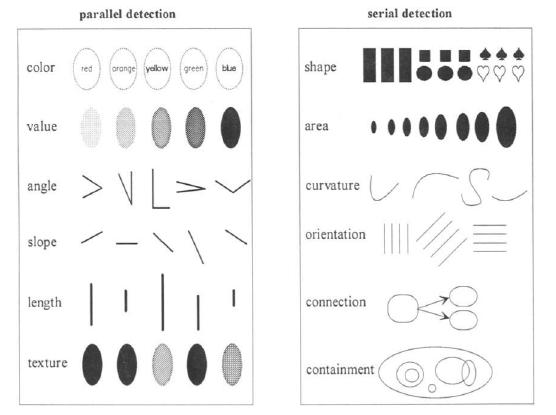
\includegraphics[width=.8\linewidth]{ParallelSerialFeatures}
\caption[Parallel and Serial Feature Detection]{Examples of features detected serially or in parallel (Chapter 6, \protect\citealt{helander1997handbook})}\label{fig:parallelSerialFeatures}
\end{figure}

Feature integration as a result of attention enables the brain to process a figure holistically. This processing is important for the most basic visual processes we take for granted, including object perception. 

\subsubsection{Object Perception} \label{ObjectPerception}
The most basic task of the visual system is to perceive objects in the world around us. This is an inherently difficult task, however, because the retina is a flat, two-dimensional surface responsible for conveying a three-dimensional visual scene. This dimensional reduction means that there are multiple three-dimensional stimuli that can produce the same visual image on the retina. This is known as the inverse projection problem - an infinite number of three-dimensional objects produce the same two-dimensional image. Less relevant to statistical graphics, but still complicating the object perception process, a single object can be viewed from a multitude of angles, in many different situations which may affect the retinal image (lighting, partial obstruction, etc). These problems mean that the brain must utilize many different heuristics to increase the accuracy of the perceived world relative to an ambiguous stimulus. 

The most commonly cited set of heuristics for object perception (and the set most relevant to statistical graphics) are known as the \emph{Gestalt Laws of Perceptual Organization} (\citealt{goldstein}, Chapter 5.2). These laws are related to the idea ``the whole is greater than the sum of the parts'', that is, that the components of a visual stimulus, when combined, create something that is more meaningful than the separate components considered individually. 

\begin{itemize}
\item \textbf{Pragnanz - the law of good figure}. Every stimulus pattern is seen so that the resulting structure is as simple as possible. 
\item \textbf{Proximity}. Things that are close in space appear to be grouped. 
\item \textbf{Similarity}. Similar items appear to be grouped together. The law of similarity is usually subordinate to the law of proximity. 
\item \textbf{Good Continuation}. Points that can be connected to form straight lines or smooth curves seem to belong together, and lines seem to follow the smoothest path. 
\item \textbf{Common Fate}. Things moving in the same direction are part of a single group.
\item \textbf{Familiarity}. Things are more likely to form groups if the groups are familiar. 
\item \textbf{Common Region}. Things that are in the same region (container) appear to be grouped together
\item \textbf{Uniform Connectedness}. A connected region of objects is perceived as a single unit.
\item \textbf{Synchrony}. Events occurring at the same time will be perceived as belonging together.
\end{itemize}

\subsubsection{Visual Memory}
We have discussed how visual stimuli are perceived and how objects are recognized; we now must examine how visual stimuli are encoded into memory. Most researchers believe that visual perceptions are encoded in an analog fashion, so that the memory of an image is closely related to the perception of that same image \citep{cognition}. Other theories suggest that visual perceptions are encoded semantically, that is, the description of a visual scene would be encoded, rather than a mental ``image" of that scene. Both theories are likely at least partially correct, but the analog encoding of visual images is more relevant to statistical graphics because the accuracty of the stored image has the potential to affect recall of the contents of that image (and thus what people remember about a particular graphic). Experimental evidence for analog encoding includes the mental rotation task, where participants must determine whether or not a figure is a rotation of a target figure, as shown in Figure \ref{fig:mentalRotation}. \citet{shepard1988mental} showed that reaction time was proportional to the angle of rotation of the stimuli, which suggests that participants were mentally rotating the figure as they would rotate a three-dimensional figure in space. 


\begin{figure}[h]\centering
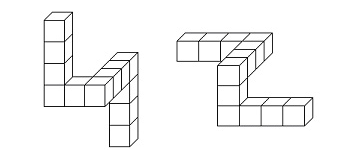
\includegraphics[width=.7\textwidth]{RotationTask}
\caption[Rotation Task]{Rotation task \protect\citep{shepard1988mental}. Are the two images the same?}\label{fig:mentalRotation}
\end{figure}

In addition, \citet{kosslyn1978visual} showed that mental representation of distances in a figure are accurate and that the time to encode those distances is proportional to the distances in the actual figure. These studies suggest that the memory of an image (statistical graphic or otherwise) is a reasonably accurate facsimile of the original image (though this is of course likely to be moderated by attention and recall ability). 

Another facet of visual memory that will be important to understanding perception and memory of statistical graphics is that the ``gist" of an image is stored along with the image. In these cases, recall ability is more consistent with the semantic encoding of images; that is, when shown an ambiguous figure (such as Figure \ref{fig:ambiguousrabbit}) and asked to describe it initially, participants could not give an alternate interpretation of the figure after the experiment was complete. In the case of  Figure \ref{fig:ambiguousrabbit}, participants who initially said the figure was a duck could not describe the figure as a rabbit later, even though the image is consistent with either interpretation. This suggests that in some cases, verbal encoding of a figure (i.e. describing it as a duck) disrupts the mental representation of the picture. This is common in other types of memories as well: when the gist of a passage is stored, the actual content of the passage is no longer accessible. In other words, we would expect that if someone had to interpret a graph, they would remember the interpretation much more strongly than the actual graph, even if that interpretation was incorrect or incomplete. 

\begin{figure}[h]\centering
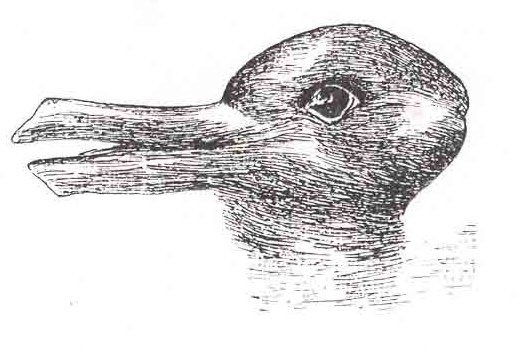
\includegraphics[width=.4\textwidth]{DuckRabbitIllusion}
\caption[Ambiguous Images]{An ambiguous image that could be either a rabbit or a duck. When participants were asked to identify the image initially, they could not provide an alternate interpretation of the figure later.}\label{fig:ambiguousrabbit}
\end{figure}

\subsubsection{Cognitive Load} Short term memory and other considerations
\todo[inline]{Add short term memory and importance of freeing up brain cells to make it easier to retain information from graphics}

The ``software" of the visual system is of course more complex than the few programs listed here, but understanding attention, object perception concepts, and how images are stored for later retrieval in the brain will make designing statistical graphics for the visual system easier and will also help with evaluating graphics based on the capabilities of the human visual system. 


\subsection{Bugs and Peculiarities of the Visual System}
We have discussed the neural ``hardware" of the visual system and some of the higher-level processing that contributes to our ability to create and understand meaning in the world around us. Occasionally, our highly tuned perceptual system fails in unusual ways due to the heuristics and algorithms that were optimized for operation in a three-dimensional world where the main tasks were hunting, gathering, and avoiding predators. We will examine three interesting results of this tuning that are important to the design of statistical graphics as we transition from the psychophysics and cognitive psychology literature to statistics and human-computer interaction literature. 

\subsubsection{Logarithmic perception} One of the earliest psychophysics researchers, Ernst Weber, discovered that the difference threshold, the smallest detectable difference between two sensory stimuli, increased proportionately with the magnitude of the stimulus. This statement, known now as Weber's Law, holds true for a large range of intensities of a number of senses. Numerically, Weber's Law is stated as 
\begin{equation}\label{weberlaw}
\frac{\triangle S}{S} = K
\end{equation}
where $K$ is a constant called the Weber fraction, $S$ is the value of the standard stimulus, and $\triangle S$ is the difference between the standard stimulus and the test stimulus. So if a participant is given a 100-g weight and a 102-g weight and can just barely tell the difference between the two, then $K=0.02$ and we would assume that the the difference between a 200-g weight and a 204-g weight would be just barely detectable as well (Chapter 1, \citealt{goldstein}). While this example concerns the ability to distinguish weight, the same law holds for the ability to distinguish sounds of different intensities as well as intensity of colors. The tendency of the brain to perceive stimuli in a logarithmic fashion is true across many perceptual domains. In fact, when kindergarden children are asked to place numbers 1-10 along a number line, they place 3 in about the middle, just as one would expect from a logarithmic perspective. This ability disappears with mathematical education, but persists in those who are not given a formal education in mathematics, indicating that our brains are naturally wired to perceive numbers logarithmically as well \citep{varshney2013we}. In some sensory domains, even the scales used to measure stimuli such as sound intensity, earthquake intensity, and frequency along the electromatic spectrum are logarithmic. Information theory suggests that logarithmic scaling provides optimal compression of information to minimize relative errors in perception while accounting for limits in our neural bandwidth. \citet{sun2012framework} showed that a bayesian model for perception would result in a model that mimics the logarithmic relationship in Weber's Law. This suggests that the logarithmic nature of human perception is a result of an heuristic that increases processing power by reducing the neural bandwidth necessary to process information through quantization of continuous information and compression of discrete information. 

From a statistical graphics point of view, then, log-transformed scales should be used instead of linear scales for continuous color scales, as this provides more information discrimination ability and mimics natural human perceptual tendencies. 

\todo[inline]{Expand this? Move? }

\subsubsection{Colorblindness and color perception}
Another common ``bug" in the visual system are mutations that change (or remove entirely) the cones in the retina. Such mutations are commonly termed ``colorblindness" and encompass many different types of mutations, shifts and deletions that affect color perception in the visual system. These mutations affect up to 5\% of the population, and are generally more common in males than they are in females, as two of the three genes producing cones are found on the X chromosome. Evolutionarily, these mutations are maladaptive for gathering plants, but may be adaptive for seeing camoflauged objects \citep{morgan1992dichromats}. In statistical graphics, however, these mutations often disrupt perception of standard color schemes used in maps, heatmaps, and divergent color scalings. Figure \ref{fig:USflag} shows the us flag as seen by those with different types of color-blindness; the red and blue hues look radically different to those with different mutations. 

\begin{figure}[h]\centering
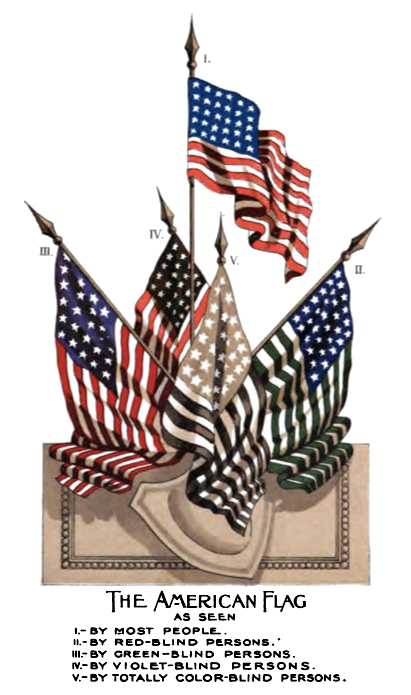
\includegraphics[width=.3\textwidth]{USflagColorBlind}
\caption[Colorblindness and US Flags]{An 1895 illustration of the US flag as seen by those with different types of colorblindness.}\label{fig:USflag}
\end{figure}

In the natural world, many strategies can be used to compensate for colorblindness; the most common of these strategies is to look for textural variation instead of color variation (which may be why camoflauged objects are easier to see), but these strategies fail when viewing abstract, constructed visual stimuli, such as graphics. Compounding this problem, the rainbow color schemes that are commonly used are particularly vulnerable to misinterpretation by colorblind viewers. Figure \ref{fig:colorblindrainbow} shows a map using a rainbow color scheme (first shown in \citet{light2004end}) and simulated images showing what that map would look like to those with missing cones (-anopia) and cones with altered wavelengths (-anomaly). These simulations show that rainbow color schemes are incredibly difficult for color-deficient individuals to read. \citet{light2004end} provides color schemes that are more appropriate for those with color deficiencies, but not all of these schemes are appropriate for all types of color blindness. \citet{silva2011using} suggest many tools to recommend appropriate color schemes for colorblind users as well as tools to preview graphics as they might look to color-deficient or colorblind users. 

\begin{figure}[h]\centering
\begin{subfigure}[b]{.4\textwidth}\centering
  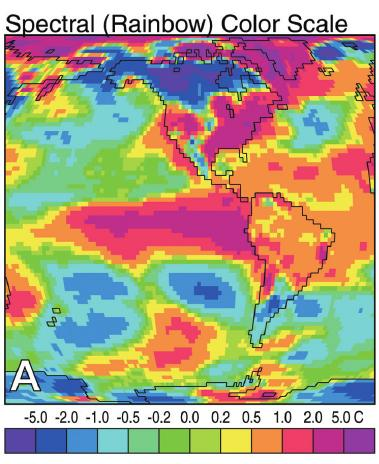
\includegraphics[width=\textwidth]{RainbowScaleOrig}
  \caption{Original Figure}
\end{subfigure}\\

\begin{subfigure}[b]{.3\textwidth}\centering
  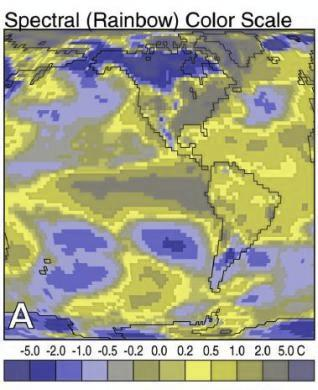
\includegraphics[width=\textwidth]{RainbowScaleOrig-protanopia}
  \caption{Protanopia}
\end{subfigure}\hfill
\begin{subfigure}[b]{.3\textwidth}\centering
  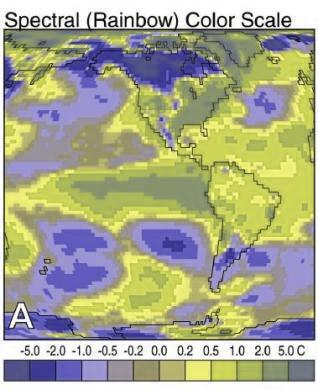
\includegraphics[width=\textwidth]{RainbowScaleOrig-deuteranopia}
  \caption{Deuteranopia}
\end{subfigure}\hfill
\begin{subfigure}[b]{.3\textwidth}\centering
  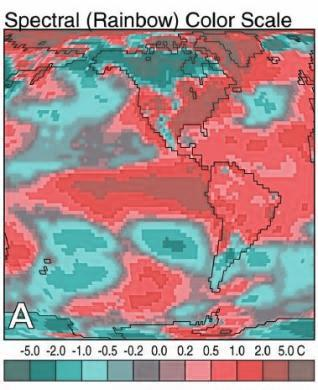
\includegraphics[width=\textwidth]{RainbowScaleOrig-tritanopia}
  \caption{Tritanopia}
\end{subfigure}\hfill

\begin{subfigure}[b]{.3\textwidth}\centering
  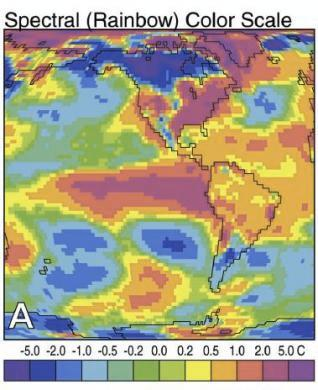
\includegraphics[width=\textwidth]{RainbowScaleOrig-protanomaly}
  \caption{Protanomaly}
\end{subfigure}\hfill
\begin{subfigure}[b]{.3\textwidth}\centering
  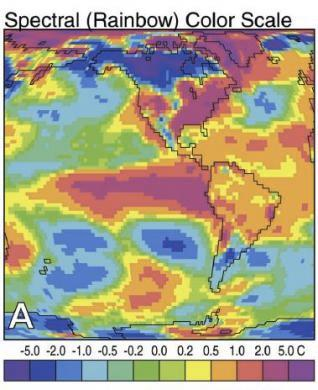
\includegraphics[width=\textwidth]{RainbowScaleOrig-deuteranomaly}
  \caption{Deuteranomaly}
\end{subfigure}\hfill
\begin{subfigure}[b]{.3\textwidth}\centering
  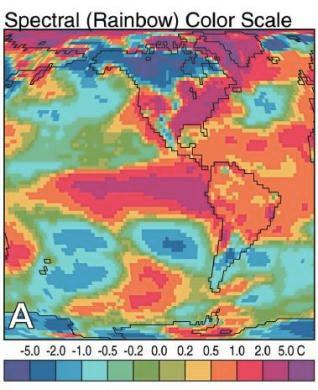
\includegraphics[width=\textwidth]{RainbowScaleOrig-tritanomaly}
  \caption{Tritanomaly}
\end{subfigure}\hfill
\caption[Colorblindness and Rainbow Color Schemes]{Rainbow color scheme with simulations of each of the three types of colorblindness in which a cone is entirely missing. The original image is from \protect\citet{light2004end}, and simulations of color deficiencies were provided by \url{http://www.color-blindness.com/coblis-color-blindness-simulator/}}\label{fig:colorblindrainbow}
\end{figure}
\comment{I can't tell a difference between the Protan* and Deuteran* pictures in Figure \ref{fig:colorblindrainbow} at all. Is that just me?}

\todo[inline]{Need to add paragraph on appropriately spaced colors and perception - i.e. green is a good color because we can see a TON of different shades of green, but we have to map to the range of colors we can discriminate. I can't find the citation, though.}

\subsubsection{Optical Illusions}
The ``software" programs presented in section \ref{Software} are generally efficient at completing everyday tasks: navigating the environment, avoiding predators (lions or cars, as the case may be), and identifying situations and objects relevant to the task at hand. As with most heuristic-based algorithms, though, these approaches produce suboptimal results when applied to more artificial tasks, such as reading statistical graphics. As such, it is important to understand where conflicts between sensation and perception may occur, so that these conflicts can be dealt with or avoided entirely. In this section, we will discuss several optical illusions and explanations for their occurence based on the visual system.

\paragraph{Physiological Illusions} The illusions shown in Figure \ref{fig:InhibitionIllusions} are illusions which occur due to the wiring of the brain. These illusions can generally be avoided, but are difficult to mitigate once they occur. 

\paragraph{Gestalt Illusions} Some illusions occur due to a conflict of gestalt principles. Two of these illusions are shown in Figure \ref{fig:GestaltIllusions}: the figure/ground illusion, and the illusory contour illusion. The figure/ground illusion depends on the color of the top and bottom edges of the picture; if the edges are black, the vase appears to be the central part of the image; if the edges are white, the faces appear to be the central part of the image. When the edges are omitted, the image seems to oscillate between the vase and the faces. This is a result of ambiguity in identifying which part of the image is the background; when the top and bottom edges are present, that cue is sufficient to resolve the illusion. The Kanizsa triangle demonstrates the Gestalt principles of good form and continuity: We perceive objects that are partially obscured by a floating white triangle, even though no such triangle actually exists. The illusory triangle produces an image that is much simpler (3 circles, a black triangle outline, and a white triangle) than the objects that are actually displayed (3 partial circles and three V shapes arranged pointing in toward a central point). In general, these gestalt principles make sense of the natural world, but when applied to artificial contexts, they occasionally produce unexpected results. 

\begin{figure}[h]\centering
\hfil
\begin{subfigure}[b]{.4\textwidth}\centering
  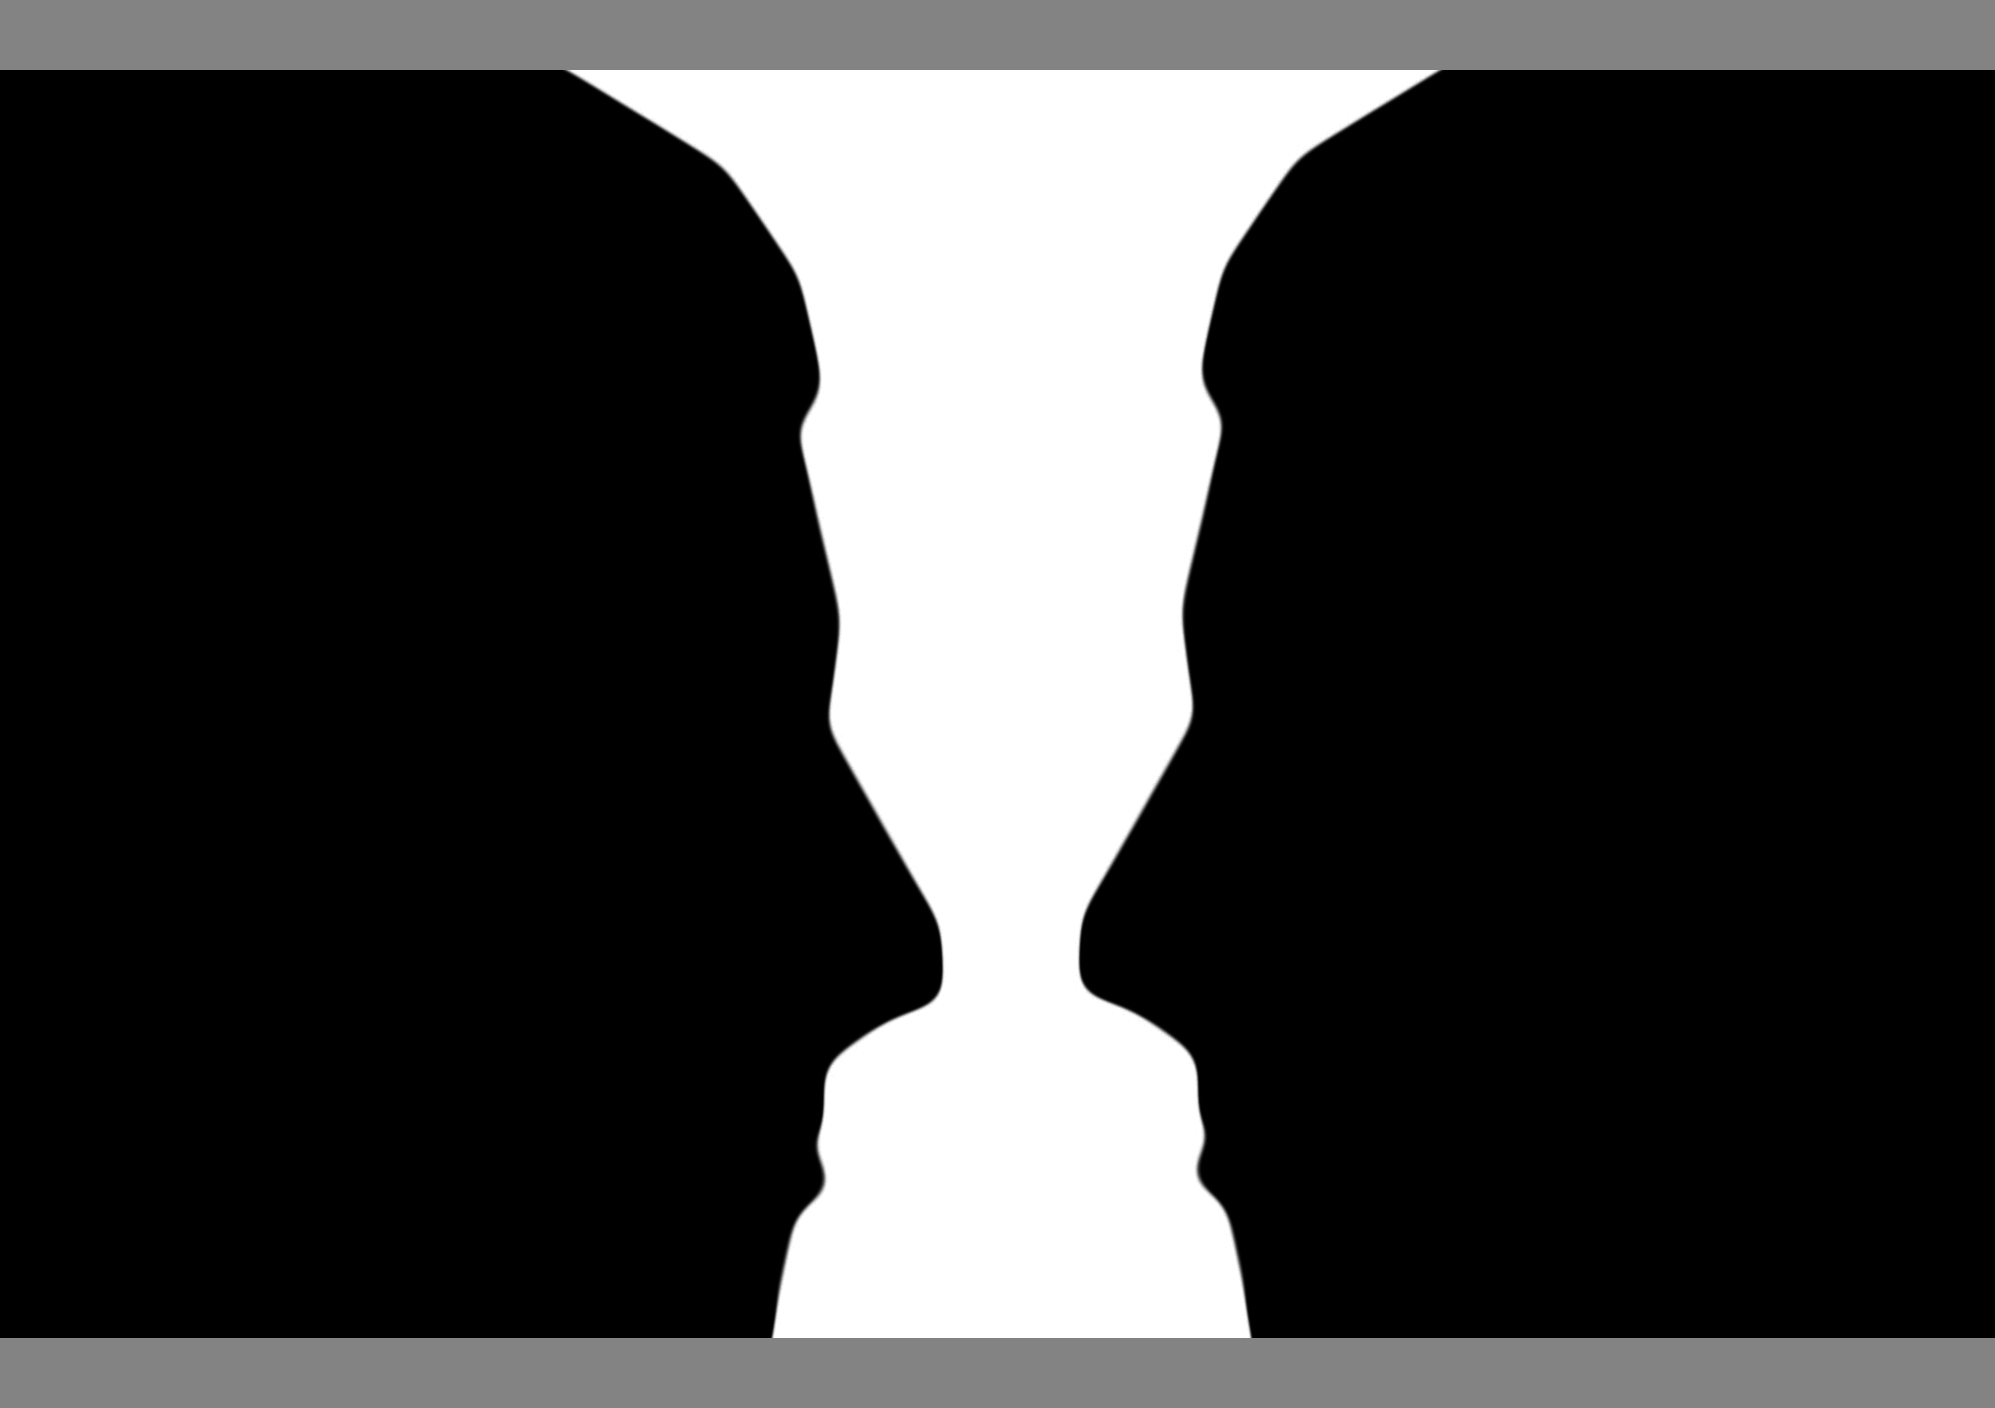
\includegraphics[width=\textwidth]{FigureVase}
  \caption{Figure-Ground Illusion}
\end{subfigure}\hfil
\begin{subfigure}[b]{.4\textwidth}\centering
  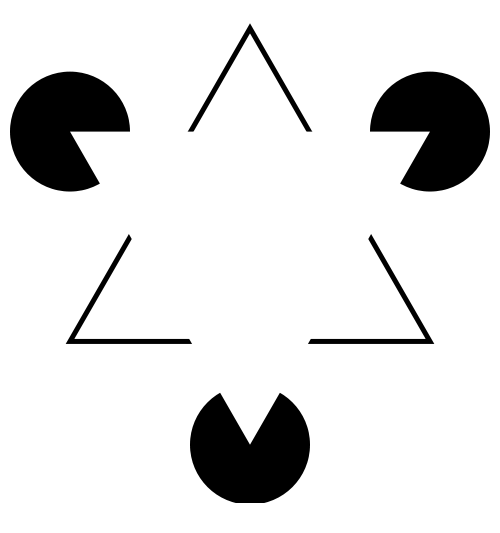
\includegraphics[width=\textwidth]{IllusoryContour}
  \caption{Kanizsa Triangle Illusion}
\end{subfigure}\hfil
\caption[Gestalt Illusions]{Illusions due to misapplied or ambiguous Gestalt rules.}\label{fig:GestaltIllusions}
\end{figure}

\paragraph{Depth illusions} Other optical illusions occur due to the optimization of the visual system for three-dimensional perception. These three-dimensional heuristics can produce unexpected or misleading results when applied to two dimensional objects. 

\begin{figure}[h]\centering
\hfil
\begin{subfigure}[b]{.4\textwidth}\centering
  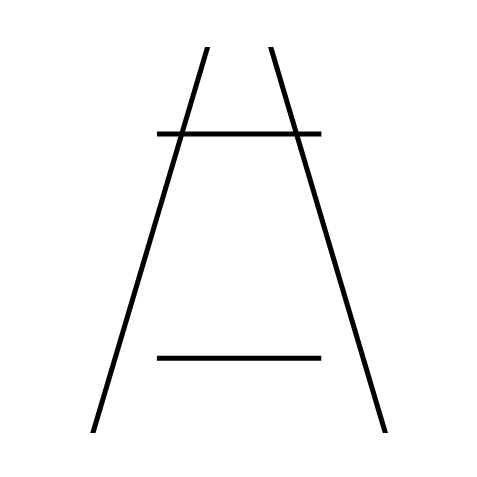
\includegraphics[width=\textwidth]{PonzoIllusion}
  \caption{Ponzo Illusion}\label{fig:Ponzo}
\end{subfigure}\hfil
\begin{subfigure}[b]{.4\textwidth}\centering
  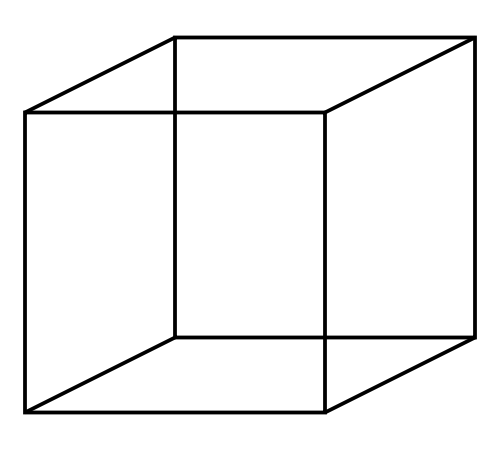
\includegraphics[width=\textwidth]{NeckerCube}
  \caption{Necker Cube}\label{fig:NeckerCube}
\end{subfigure}\hfil

\hfil
\begin{subfigure}[b]{.4\textwidth}\centering
  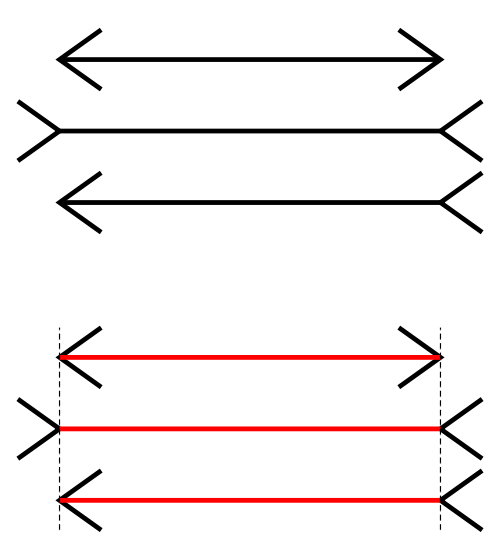
\includegraphics[width=\textwidth, angle=90]{MullerLyer}
  \caption{Muller-Lyer Illusion}\label{fig:MullerLyer}
\end{subfigure}\hfil
\begin{subfigure}[b]{.4\textwidth}\centering
  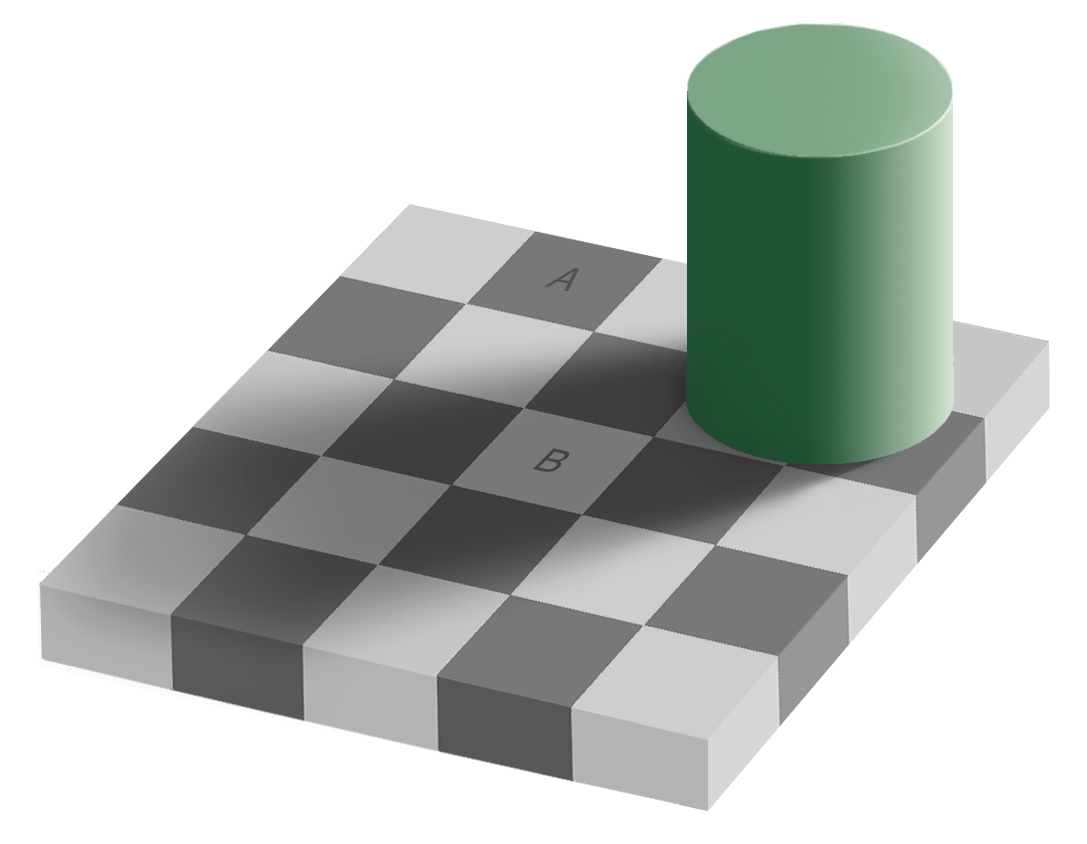
\includegraphics[width=\textwidth]{CheckerShadow}
  \caption{Color Constancy Illusion}\label{fig:ColorConstancy}
\end{subfigure}\hfil

\caption[Depth Illusions]{Illusions due to misapplied depth perception.}\label{fig:DepthIllusions}
\end{figure}
Figure \ref{fig:DepthIllusions} contains four of the more interesting optical illusions that result from ambiguous figures that trigger depth cues. The Ponzo illusion (Figure \ref{fig:Ponzo}) suggests that the top line is longer than the bottom line, because of the implied convergence of the two vertical lines (to understand the natural scenario behind this illusion, consider railroad tracks converging at the horizon). The Necker Cube, shown in figure \ref{fig:NeckerCube}, can be seen such that the top-right face is closest to the viewer or alternately such that the bottom-left face is closest to the viewer. Due to the ambiguity in the image, it will often seem to "flip" when the viewer loses focus on the image momentarily. The Muller-Lyer illusion (Figure \ref{fig:MullerLyer}) is generally believed to result from misapplied depth cues as well - the left-most image would occur in nature as the exterior corner of a building, the middle image would occur when viewing an interior corner of the same building, further away from the viewer. As a result of the illusion, the middle line appears to be longer than the first or third lines. Figure \ref{fig:mullerlyerhouse} shows the first two parts of the illusion in a context which removes the ambiguity through additional depth cues. The additional cues result in the resolution of the illusion. Finally, the color constancy illusion shown in Figure \ref{fig:ColorConstancy} suggests that the square marked A is much darker than the square marked B, even though the two squares are the same color. This illusion results from our experiences with depth and shadows: square B is perceived to be the same color as the lighter-colored squares outside the shadow, while square A is perceived to be the same color as the other dark squares in the tile pattern, regardless of the actual color due to the shadow. 

\begin{figure}[h]\centering
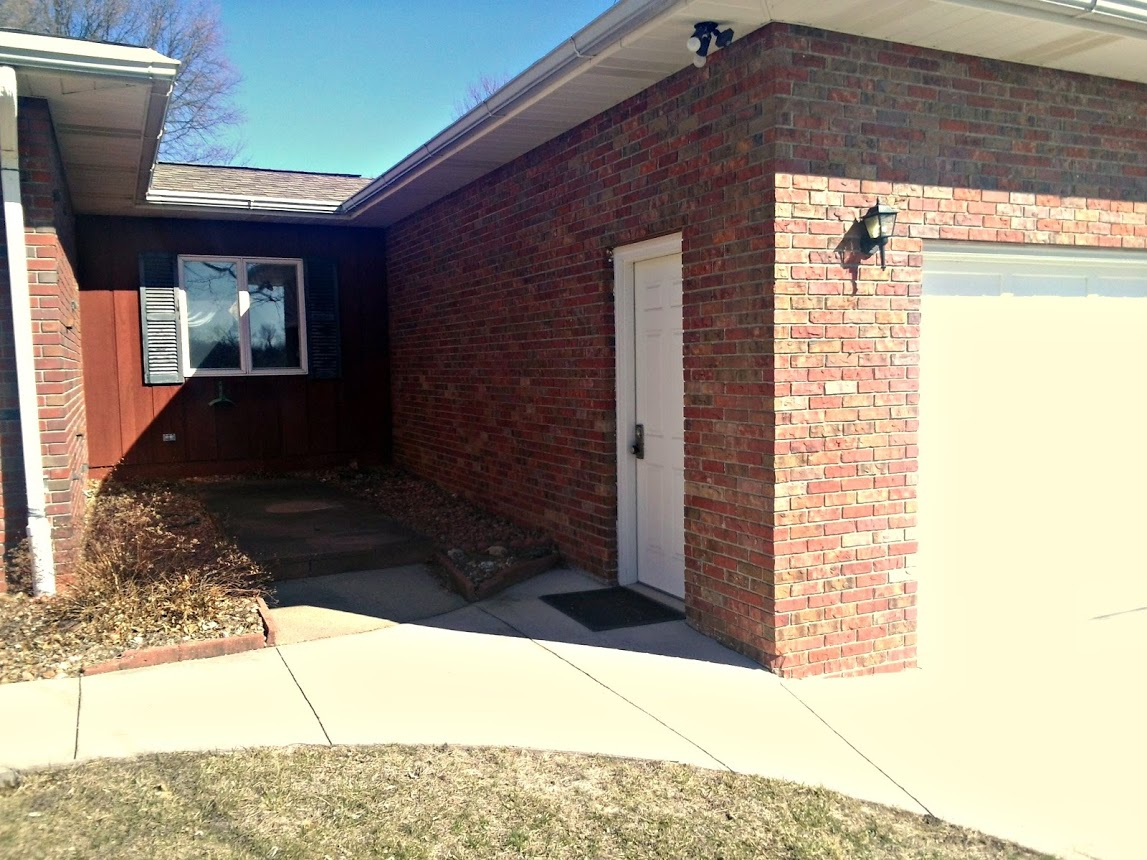
\includegraphics[width=.5\textwidth]{mullerlyerhouse}
\caption[Muller Lyer Illusion]{The Muller-Lyer illusion in a non-ambiguous three-dimensional context.}\label{fig:mullerlyerhouse}
\end{figure}

\section{Statistical Graphics}
\subsection{Low-level perception of graphics}\label{LowLevelGraphics}
Healey's preattentive feature integration stuff
\subsection{Higher-level graphical perception}\label{HighLevelGraphics}
\begin{itemize}
\item Cleveland \& McGill
\item Heuristic guidelines i.e. Kosslyn and Tufte
\item Grammar of graphics allows us to test graphics which display the same information in different ways for comparable accuracy
\end{itemize}
Emphasize the low-level stuff vs. the higher-level stuff that focuses on preattentive information (i.e. not what we care about) and the gap in the middle where graphics are tested in more practical scenarios.

\subsection{Optical illusions and statistical graphics}
three-dimensional context, other ways to trigger optical illusions with graphics. Importance of being aware of the heuristics the brain uses so that problematic graphics can be avoided. 

\subsection{Interactive graphics?} 
Not sure if this should be a subsection, but graphics that respond to human interaction violate the two-dimensional graphic paradigm somewhat, which means there are a whole 'nother set of issues to consider... motion illusions, grouping, etc.

\section{Testing Statistical Graphics}
Methodology for testing graphical perception in humans. Talk about masking, the power of suggestion, habituation, etc. as well as paradigms - search and find, response time, numerical judgments, signal detection, eye tracking. 
\begin{itemize}
  \item Tukey
  \item Cleveland \& McGill
  \item Lineups
\end{itemize}




\graphicspath{{Figure/sineIllusion/}{Images/sineIllusion/}}
\renewcommand{\floatpagefraction}{.99}

\newcommand{\range}[1]{{\text{range}\left(#1\right)}}
\newcommand{\s}[2]{{_{#1}s^{ #2}}}
\newcommand{\atan}[1]{\text{atan}\left({#1}\right)}
\newcommand{\xR}{\mathbb{R}}









\chapter{SIGNS OF THE SINE ILLUSION -- WHY WE NEED TO CARE}
%% Abstract
% Graphical representations have to be true to the data they display. Computational tools ensure this on a technical level. But we also need to take `flaws' of the human perceptual system into account. The sine illusion provides an example where human perception leads to systematic bias in the assessment of the optical stimulus, with a particularly notable impact on perception of time-series data with a seasonal component. In this paper, we discuss the reasons for the illusion and various strategies  useful to break the illusion or reduce its strength. We demonstrate the presence of the illusion in real-world and theoretical situations. We also present data from a user study which demonstrate the dramatic effect the sine illusion can have on conclusions drawn from displayed data.


\section{Introduction}
Graphics are powerful tools for summarizing large or complex data, but they rely on the main premise that any graphical representation of the data has to be ``true'' to the data (see e.g. \citet{tufte, wainer:2000, robbins:2005}). That is, a measurable quantity of a graphical element in the representation has to  directly reflect some aspect of the underlying data. Generally, we see a lot of discussion on keeping true to the data in the framework of (ab)using three dimensional effects in graphics. \cite{tufte} goes as far as defining a {\it lie-factor} of a chart as the ratio of the size of an effect in the data compared to the size of an effect shown, with the premise that any large deviations from one indicate a misuse of graphical techniques. Computational tools help us ensure technical trueness -- but this brings up the additional question of how we deal with situations that involve innate inability or trigger learned misperceptions in the audience. In this paper we want to raise awareness for one of these situations, show that it occurs frequently in our dealings with graphics and provide a set of strategies for solving or avoiding it.




\begin{figure}[h!tbp]\centering
\begin{subfigure}[b]{.45\textwidth}
  \centering
  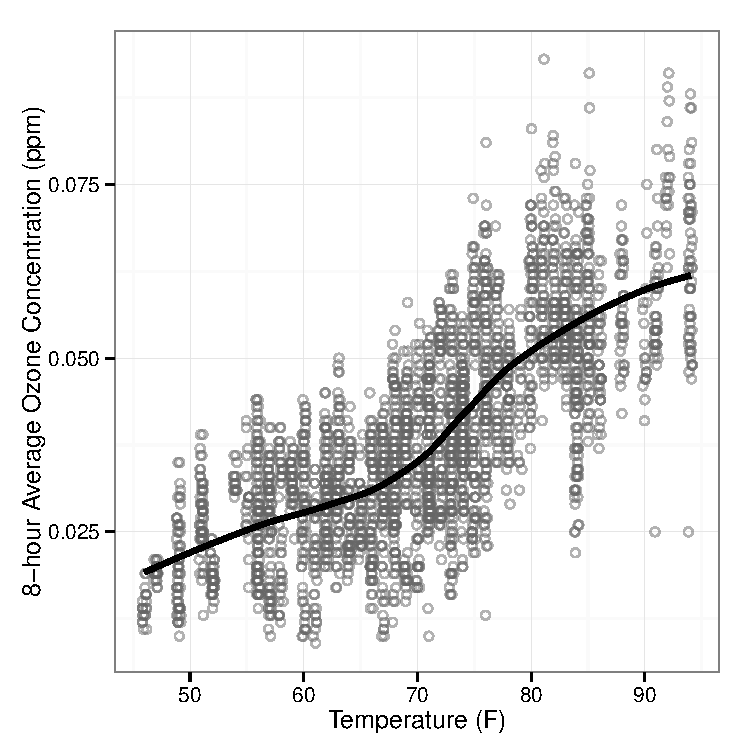
\includegraphics[width=\textwidth]{fig-example1}
  \caption[Scatterplot of Ozone and Temperature in Houston, 2011.]{\small Scatterplot of Ozone and Temperature in Houston, 2011. A loess fit is overlaid to show the overall trend.  \label{fig:example1}}
\end{subfigure}\hfill
\begin{subfigure}[b]{.45\textwidth}
  \centering
  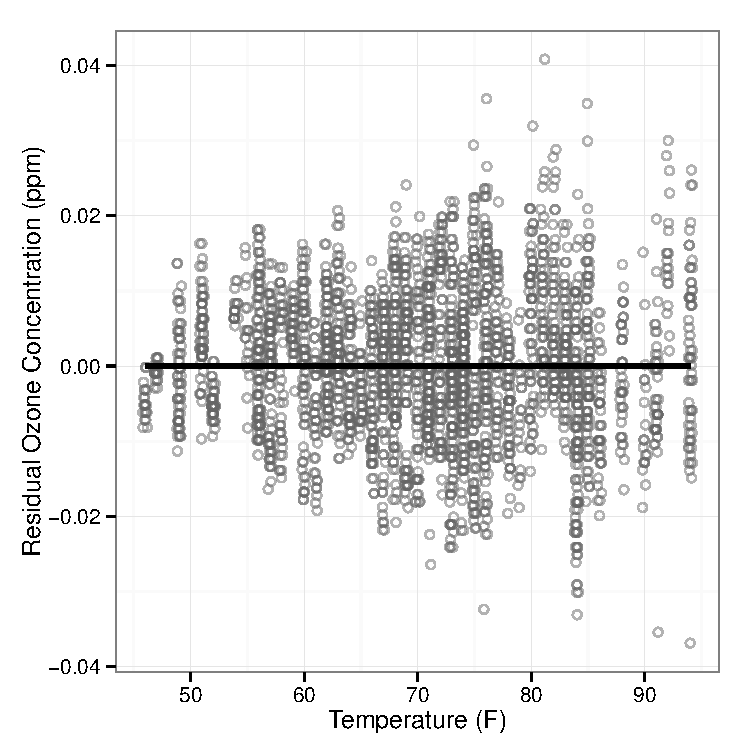
\includegraphics[width=\textwidth]{fig-example2}
  \caption[Residual Ozone]{\small Scatterplots of Ozone and Temperature de-trended according to the loess fit in (a). \\ \phantom{text to get to the next line}
  \label{fig:example2}}
\end{subfigure}
\caption[Scatterplots of Ozone and Temperature in Houston, 2011]{\label{fig:exampleFull1} Scatterplots of Ozone and Temperature in Houston, 2011. The increase in variability over the temperature range is more pronounced in the de-trended plot on the right.}
\end{figure}

As a first example let us consider the relationship between ozone concentration and temperature. Ozone concentrations were measured from 21 locations in the Houston area \citep{epa}, and temperature data is provided by the NCDC \citep{noaa} site at Hobby International Airport, located near the center of Houston. 

Figure~\ref{fig:example1} shows daily measurements of 8-hour average ozone concentration and temperature at several sites in Houston, for days in 2011 with temperatures above $45^\circ$F  and dew points of less than $60^\circ$F. 
A loess smooth line is added for reference. 
These types of plots are often used to give an overview of the relationship between two variables. The trendline summarizes this relationship, while the points show raw measurement to allow an assessment of the overall size of the data, the amount of (marginal) variability presented, as well as the (conditional) variability along the trendline. It is the latter task that we cannot satisfactorily complete. While
we might agree that there is an increase in variability of ozone concentrations for temperatures above $80^\circ$F, we will not doubt homogeneity  elsewhere based on figure~\ref{fig:example1}. 


This evaluation changes when considering figure~\ref{fig:example2}: the scatterplot shows a loess based de-trended residual of temperature. A previously almost invisible increase in variability of ozone measurements with increasing temperatures now becomes apparent.

This phenomenon, caused by the change in the slope of the trend line,  is  known as the  {\it sine illusion} in the literature on cognition and human perception  or {\it line width illusion} in the statistical graphics literature. 

The illusion is a frequent occurrence in statistical graphics, and  displays should therefore be thoughtfully considered to minimize its effect visually and acknowledge its influence. 
In the cognitive literature, \citet{day:1991} first documented the illusion in the context of vertical lines along a sinusoidal curve. Figure~\ref{fig:original} shows a sketch of this: line segments are centered evenly spaced along the curve. Line segments are of equal length but appear longer in the peaks and troughs due to the illusion. The parameters that influence the strength of the illusion are the amplitude of the curve and the length of the line segments. As the length of the line segments increases,  the apparent difference in the length of the line segments decreases. Any modification that increases the change in slope under which the curve appears, such as an increase in the amplitude of the curve or a more extreme aspect ratio, reinforces the apparent difference in line lengths. 







\begin{figure}[hbtp]
\centering
\begin{knitrout}
\definecolor{shadecolor}{rgb}{0.969, 0.969, 0.969}\color{fgcolor}

{\centering 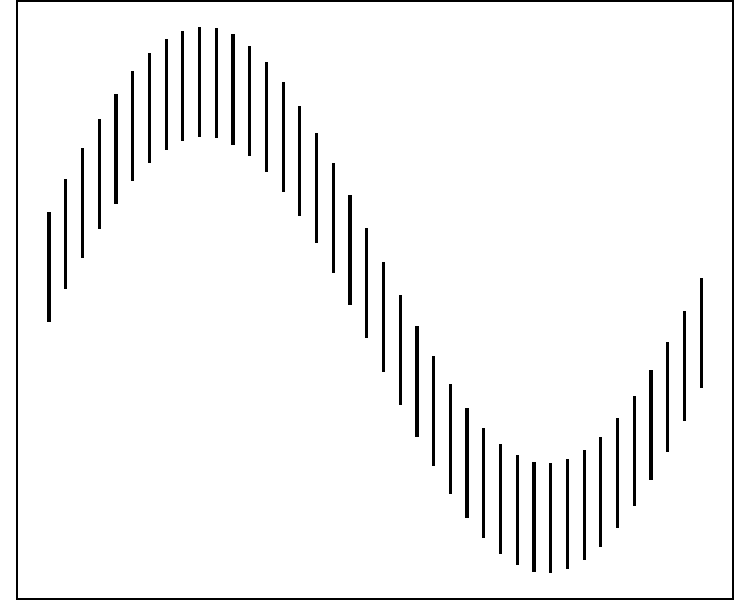
\includegraphics[width=.4\textwidth]{../Figure/sineIllusion/fig-original} 

}



\end{knitrout}

\caption[The original sine illusion]{The original sine illusion, demonstrated on evenly spaced vertical lines centered around a sinusoidal curve of $f(x) = \sin(x)$. The lines in the peak and trough of the curve appear to be longer than in the other regions.\label{fig:original}}
\end{figure}

More recently the illusion has been shown in non-sinusoidal curves \citep{cleveland:1984, schonlau:2003, robbins:2005, marie:2013}, but the underlying effect seems to be the same, in the sense that the illusion is not triggered by the periodic nature of the underlying trendline but only by  changes to its slope. Figure \ref{fig:twoillusions-simulation} shows three panels, which all exhibit the illusion. From left to right, the trend stems from (a) a periodic function, (b) a periodic component added to an exponential function, and (c) an exponential function on its own.
While all three graphs seem to show nonconstant variance along the main trend; in reality, it is constant. Clearly, the illusion does not rely on the periodicity of the function for which it was named, but is a symptom of the change in curvature that comes with the periodicity.

\begin{figure}[h!tbp]\centering
\begin{subfigure}[b]{.31\textwidth}
  \centering
\begin{knitrout}
\definecolor{shadecolor}{rgb}{0.969, 0.969, 0.969}\color{fgcolor}

{\centering 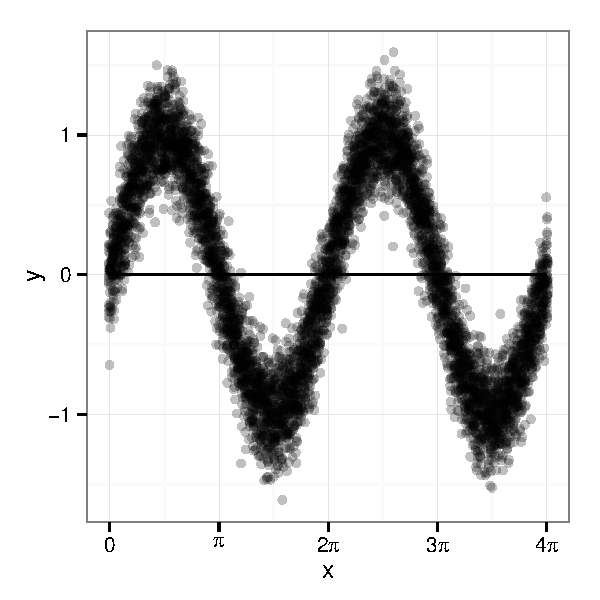
\includegraphics[width=\textwidth]{../Figure/sineIllusion/fig-simulation1Sine} 

}



\end{knitrout}

  \caption{\small Seasonality, No Trend}
  \label{simulation1}
\end{subfigure}
\begin{subfigure}[b]{.31\textwidth}\centering
\begin{knitrout}
\definecolor{shadecolor}{rgb}{0.969, 0.969, 0.969}\color{fgcolor}

{\centering 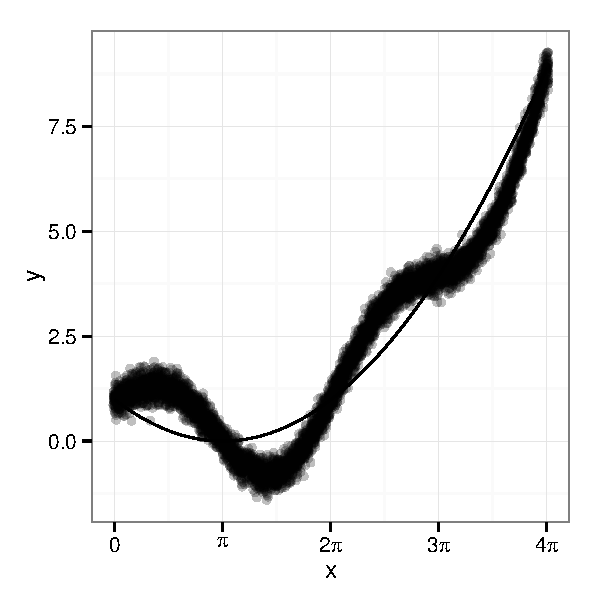
\includegraphics[width=\textwidth]{../Figure/sineIllusion/fig-simulation1Sine2} 

}



\end{knitrout}

  \caption{\small Seasonality and Trend}
  \label{simulation2}
\end{subfigure}
\begin{subfigure}[b]{.31\textwidth}\centering
\begin{knitrout}
\definecolor{shadecolor}{rgb}{0.969, 0.969, 0.969}\color{fgcolor}

{\centering 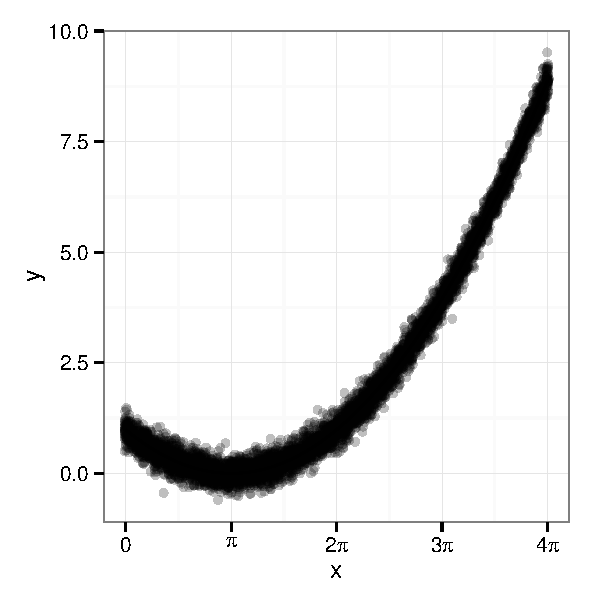
\includegraphics[width=\textwidth]{../Figure/sineIllusion/fig-simulation1Sine3} 

}



\end{knitrout}

  \caption{\small Trend, No Seasonality}
  \label{simulation3}
\end{subfigure}
\caption[Trend, seasonality, and the sine illusion]{Set of three scatterplots of simulated data with constant variance. Plot (a) shows seasonality without any underlying trend, (b) shows seasonality superimposed on a quadratic trend, and (c) shows a quadratic trend without seasonality. Though all three sets of simulated data have constant variance, none of the variances appear constant due to the sine illusion.}\label{fig:twoillusions-simulation}
\end{figure}

Next, we give an overview of the perceptual and statistical literature regarding this illusion.
\subsection{The Sine Illusion in Statistical Graphics}\label{statisticalgraphics}\hfill\newline
The sine illusion demonstrated in figures \ref{fig:exampleFull1} and \ref{fig:original} has been frequently noted in statistical graphics, though usually not as an optical illusion. Rather, the problem is typically identified as the difficulty of visually subtracting two curves, and the resulting erroneous conclusions when this process goes awry. Figure \ref{fig:playfair-debt} presents the possibly oldest example of this common phenomenon \citep{playfair, playfair2}: Playfair's chart of the balance of trade between England and the East Indies shows time series of the trade value for imports  and exports between the countries in the 18th century. The shaded area on the chart is named ``balance against England", suggesting that the difference between the lines is of main importance. This difference in trading values is encoded as the difference between the lines along the vertical axis. However, the vertical distance  between  two lines provides a  much less visually salient cue than the orthogonal width between the lines. This results in  an underestimation \citep{cleveland:1984} of the difference in trades around 1763, which is of a much higher (about 1.5 fold) magnitude as around 1770, but appears much smaller. In more modern visualizations, bivariate area charts and ``stream graphs'' \citep{stackedgraphs} commonly produce the illusion (see an example at \url{http://bl.ocks.org/mbostock/3894205}). 

\begin{figure}[h!tbp]
\centering
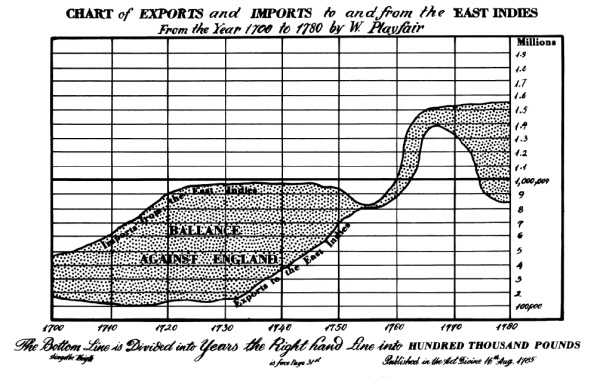
\includegraphics[keepaspectratio=TRUE,width=.7\textwidth]{PlayfairExportImports}
\caption[Imports to and Exports from the East Indies in the 1700s]{Playfair's graph of exports to and imports from the East Indies demonstrates that the line width illusion is not only found on sinusoidal curves but is present whenever the slope of the lines change dramatically. The increase in both imports and exports circa 1763 does not appear to portray as large of a deficit as that in 1710, even though they are of similar magnitude.}
\label{fig:playfair-debt}
\end{figure}

\subsection{Perceptual Explanations for the Sine Illusion}\label{perceptualexplanations}\hfill\newline
While not thoroughly examined in the sensation and perception literature, the sine illusion has been classified as part of a group of geometrical optical misperceptions  related to the M\"uller-Lyer illusion \citep{day:1991} or the Poggendorf illusion \citep{poggendorf}, which puts the illusion into the framework of context-based illusions. \citet{day:1991} suggest that the sine illusion occurs due to misapplication of perceptual experience with the three-dimensional world to a two-dimensional ``artificial" display of data.  

Experience with real-world objects suggests that the stimulus of figure~\ref{fig:original} is very similar to a slightly angled top view of the 3-dimensional figure of a strip or ribbon describing waves in a third dimension, such as e.g.~a road does on rolling hills. This is sketched out in figure~\ref{ribbon1}. Our experience suggests immediately that changes in the width of the road are unlikely and resolves the illusion. While figure~\ref{ribbon1} shows the line segments slightly angled towards each other, figure \ref{ribbon2} shows a variation of the same plot with a  vanishing point set further away from the viewer. This makes the line segments almost parallel to each other and therefore more closely resembles the sketch of figure~\ref{fig:original}, in which the sine illusion was originally presented.

%By treating the graph as a two-dimensional projection of a three-dimensional figure, the illusion disappears and the line widths seem once more to be constant.


% Figure \ref{fig:ribbon-illusion} shows a possible three-dimensional context for the classical sine illusion; two ribbons are shown at varying perspective strengths. \todo[inline]{OK, we need to slow down here, but I'm not sure how to say it. That's why I'm asking all these questions.}
% \todo[inline]{How do the perspective plots relate to the illusion - in words. I can see it, but we need to describe it in the text as well. }
% \todo[inline]{Does the 3d perspective resolve the illusion?}
% 
% \todo[inline]{What is the difference between the first and the second perspective plot?}
% The first appears more natural \todo[inline]{What do you mean by more 'natural'?}, but the second still appears three-dimensional \todo[inline]{Why?} and is much closer to the sine illusion stimuli \todo[inline]{Why is it closer?}  with added shading. 

\begin{figure}[h!tbp]\centering


\begin{subfigure}[t]{.49\textwidth}\centering
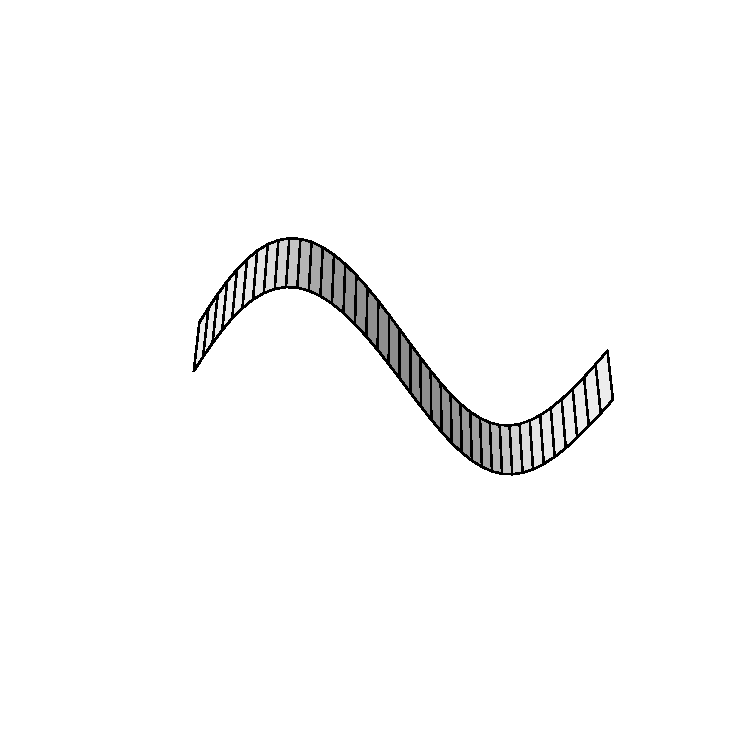
\includegraphics[width=\textwidth, keepaspectratio=TRUE, trim=0in 1.5in 0in 1.5in]{fig-ribbon-illusion1}
\caption{Perspective plot of sine illusion\label{ribbon1}}
\end{subfigure}
\begin{subfigure}[t]{.49\textwidth}\centering
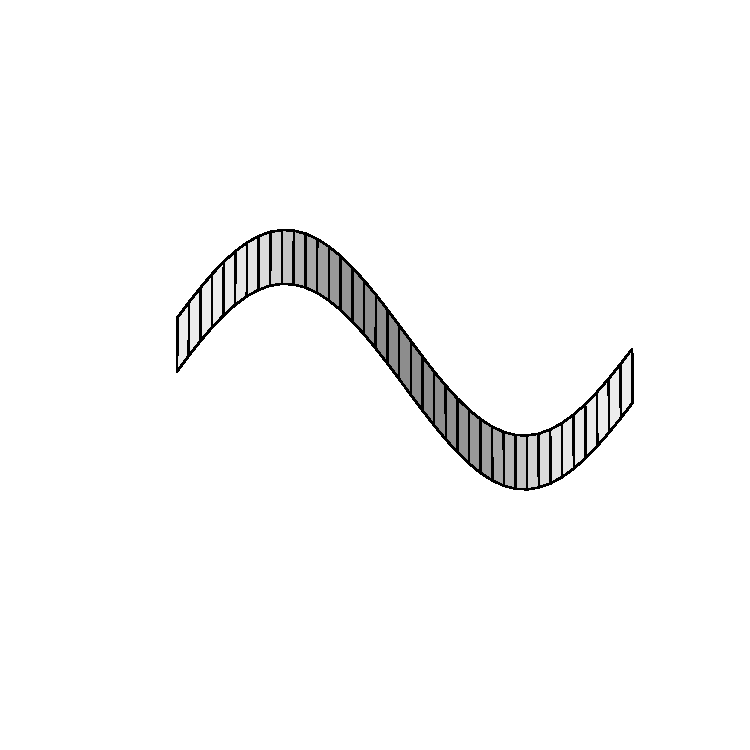
\includegraphics[width=\textwidth, keepaspectratio=TRUE, trim=0in 1.5in 0in 1.5in]{fig-ribbon-illusion2}
\caption{Perspective plot, vanishing point near infinity.\label{ribbon2}}
\end{subfigure}
\caption[Three-dimensional origins of the sine illusion]{Two different perspective projections of the same data responsible for the sine illusion. The first projection angles the lines and appears more natural, but the second projection suggests that the lines do not need to be angled to create the same three-dimensional impression.\label{ribbon}}
\end{figure}





\begin{figure}
\centering
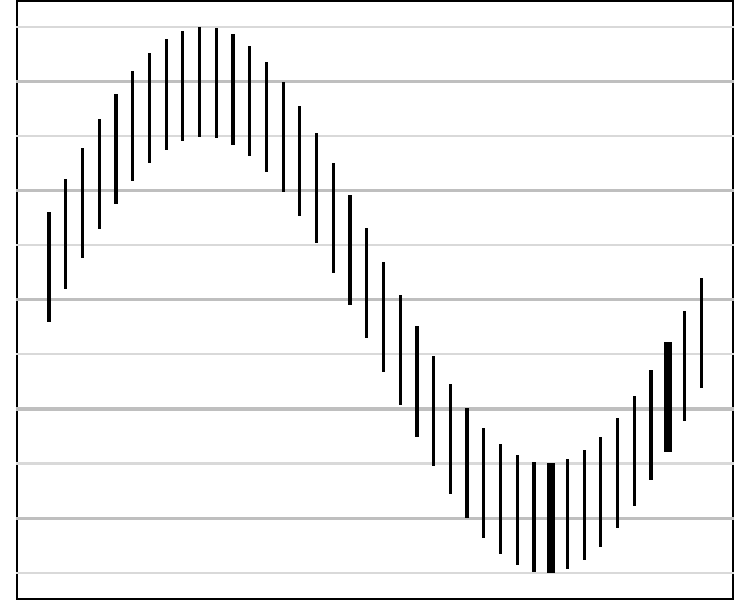
\includegraphics[width=.4\textwidth]{fig-originalgrid}
\caption[Contextual origins of the sine illusion]{\label{fig:original-grid} The sine illusion with two individual lines highlighted. Horizontal grid lines do not help  to resolve the illusion, even though they provide a clear basis for comparison of line lengths. Readers are much better at assessing the length of the two singled out line segments; they are equal.}
\end{figure}

Recreating the three-dimensional context of the sine illusion might resolve the distortion, even if increasing the dimensionality of a graph is generally not recommended \citep{tufte, cleveland:1984} (though \citet{spence:1990} suggests that in certain cases additional dimensions are not misleading). While creating a three-dimensional projection of two-dimensional data might counteract the illusion, the process of projecting the data accurately into a higher dimension is not simple. The projection that best resolves the illusion likely is highly subjective and influenced by choices of angle and color gradient for depth cues. As there is not a single three-dimensional projection that corresponds to the two-dimensional data, this approach would only produce further visual ambiguity.
%and would also lead to distortions and instability in the visual display. In particular, there does not seem to be an simple guideline for determining the projection angle or color gradient  to create the illusory depth to remove the optical illusion. 

%That is, the illusion breaks down if the visual heuristic is pre-empted by an attempt to view the graph as if it were three dimensional or if each piece is considered without the surrounding context. 
Further complicating the situation, the illusion itself is insidious -- we trust our vision implicitly, to the point that when we understand something, we say ``I see''. This trust in our visual perception is seldom called into question, for our perception is optimized for interaction with a three-dimensional world. Artificial two-dimensional situations (such as graphs and pictures) may accurately represent the data and still produce a misleading perceptual experience.

The contextual cues of the overall trend are critical to the sine illusion's effect;  the illusion  only  holds when a substantial portion of the graph is considered simultaneously, which triggers our innate ability of perceiving one whole rather than the individual parts it consists of (principle of grouping; \citet{wolfe2012sensation}).
%without regard to the perceptual mechanisms at play. 
Considering only two line segments at a time resolves the illusion. The bold lines in figure~\ref{fig:original-grid} are clearly of the same length.  Comparisons of individual line lengths is visually a fairly simple task, and is done with a relatively high accuracy \citep{cleveland:1984}. 
\citet{day:1991} contains a more thorough discussion of how much surrounding context is required for the illusion to persist. 
%The illusion arises when sufficient context is available to induce an ambiguously three-dimensional figure.

%\FloatBarrier
\subsection{Geometry of the Illusion}\hfill\newline
%We have previously alluded to the fact that the sine illusion depends on the change in the slope of the underlying function; what follows is a geometric explanation of why this occurs. 
%Our perceptual system is particularly well optimized for three dimensions; in figure~\ref{fig:original}  this leads us to perceive the  shortest line between the top and bottom curves as the distance between the curves, i.e. the {\it orthogonal} width,  rather than the vertical distance. 
In figure~\ref{fig:original} we have seen that the our preference in evaluating line width is to assess {\it orthogonal} width rather than the difference along the vertical axis. 
Figure~\ref{fig:OrthogonalWidth} demonstrates the change in orthogonal width as the slope of the line tangent to the graph of $f$ changes; these changes correspond to our perception of apparent line length. 


\begin{figure}[h!tbp]
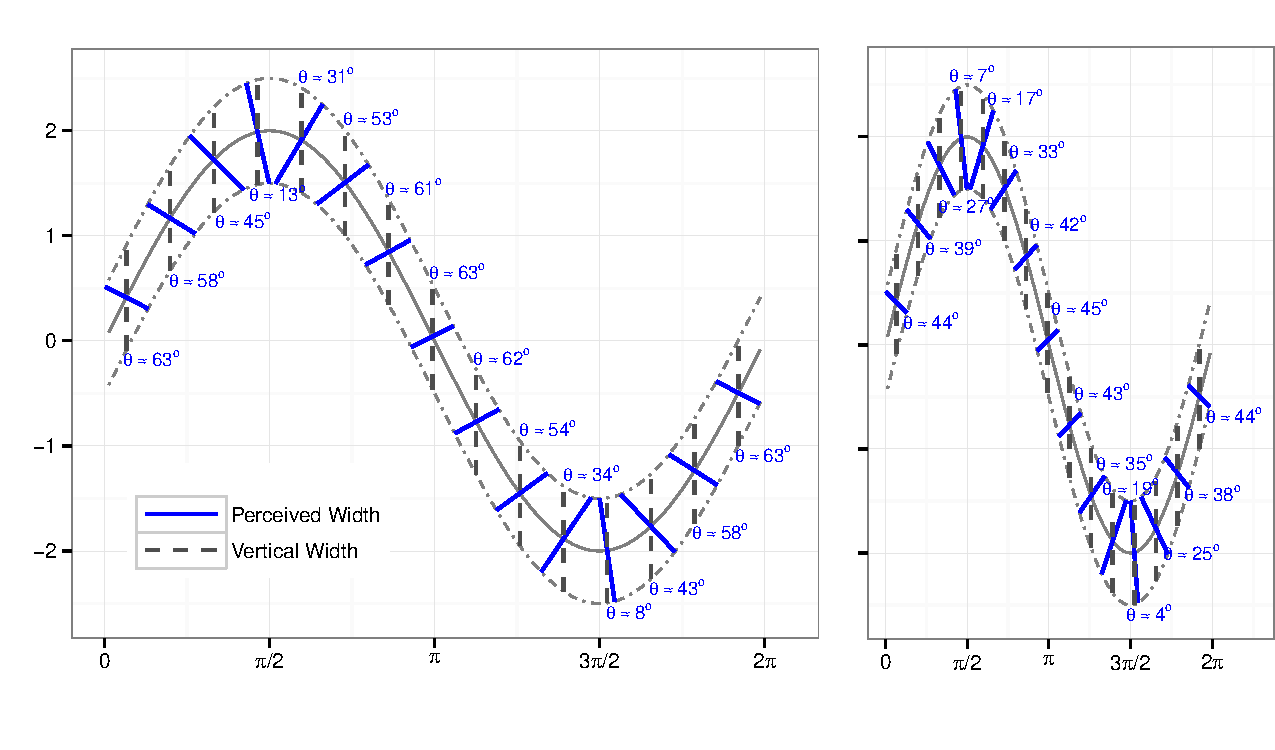
\includegraphics[width=.9\textwidth, keepaspectratio=TRUE]{fig-transform-illustration}
\centering
\caption[Geometry of the sine illusion]{\label{fig:OrthogonalWidth} The sine illusion with lines orthogonal to the tangent line at $f(x)$. The perception that the vertical length changes with $f(x)$ corresponds to changes in actual orthogonal width due to the change in the visual (plotted) secant angle. The strength of the perceptual effect depends in part on the aspect ratio of the graph, as shown in the second image, which has an aspect ratio of 2 compared to the first figure's aspect ratio of 1. This correspondingly multiplies the strength of the effect by 2. 
}
\end{figure}
%Secants and vertical lines are both shown  in figure~\ref{fig:OrthogonalWidth}. 
The illusion is most pronounced in regions where the angle between the orthogonal  and the vertical line is large. Changes to the aspect ratio therefore have a major impact on the strength of the sine illusion. Any change that alleviates the difference between perceived width and the perpendicular width, such as banking to 45$^\circ$ \citep{cleveland:88}, will alleviate the effect but not completely overcome it. 
The perceived length of the vertical line changes with the angle of the line perpendicular to the slope of $\sin(x)$, suggesting that the sine illusion stems from a conflict between the visual system's perception of figure width and the mathematical judgement necessary to determine the length of the vertical lines. 




Our preference for assessing figure width based on the orthogonal width suggests that the underlying illusion may be a function of geometry rather than some unknown visual or neural process that occurs subconsciously. In this  case it may be  possible to correct the graphical display for the illusion to minimize its misleading effect. A geometrical correction that  --at least temporarily-- counteracts the illusion would be a valuable tool in visual analysis, as this illusion very persistently affects our judgment of very common tasks  such as e.g.~the assessment of conditional variability of data along a trend line.

Simply raising people's awareness of the presence of this illusion is not enough,
as it is incredibly difficult, if not impossible, to overcome this illusion even when we are aware of its presence: our brains simply cannot ``un-see" it. 

What follows is a compilation of several approaches to correct for or mitigate the effect of the illusion. Our primary intention here is to demonstrate the persaviness of the illusion is and the extreme measures necessary to remove its effect. 
% do not change this to its'

\section{Breaking the Illusion}
The sine  illusion is caused by a conflict between vertical width, which is the width that we want onlookers to assess visually, and orthogonal width, which is the width that the onlooker perceives. This difference can be expressed as a function in the slope of the underlying trend line. This provides the basis for adjusting the vertical width for the perceived orthogonal width. 

We consider the following three approaches:  
\begin{enumerate}
\item separating the trend and the variability, 
\item transformation of $x$: adjusting the slope to be constant by reparametrizing the $x$ axis, and
\item transformation of $y$: adjusting $y$ values to make conditional variability  appear correctly by adjusting accordingto orthogonal width. 
\end{enumerate}
Each of these ideas is discussed in more detail in this section.

\subsection{Trend Removal}
% \newdo{Emphasize that multiple plots imply higher cognitive load (Wainer 1984) and that good  charts usually have to answer multiple questions.}
\citet{cleveland:1984, cleveland:1985} discuss the perceptual difficulty of judging the difference between two curves plotted in the same chart, and alternatively, recommend to display the difference between the two curves directly. This is in line with  recommendations  for good graphics to `show the data' rather than make the reader derive some aspect of it (e.g. \citet{wainer:2000}). In particular, de-trending data to focus on residual structure is the generally accepted procedure for assessing model fit. 
 Figure \ref{fig:cleveland-figure}(a) shows a scatterplot of data with a trend. A loess smooth is used to estimate the trendline. A visual assessment of variability along this trendline
might result in a description such as `homogeneous variance or slightly increasing variance for  negative $x$, followed by a dramatic decrease in vertical variability for positive $x$'.  
Once the residuals are separated from the trendline as shown on the right hand side of the figure, it becomes apparent that this first assessment of conditional variability was not correct, and the decreasing variance along the horizontal axis becomes visible.
 
While the illusion is not apparent when trend line and variability in the  residual structure are shown separately, the separation 
makes it  more difficult to evaluate the overall  pattern in the data, as we  must base any judgment on two charts; either by combining information from two graphs or by mentally re-composing the original graph (at which point, the sine illusion becomes a factor). To minimize cognitive demands we ideally want to tell the whole story with a single graph, in particular because in many situations we may not be able to show multiple graphs. 



\begin{figure} \hfill
\begin{subfigure}[b]{.45\textwidth}
  \centering
  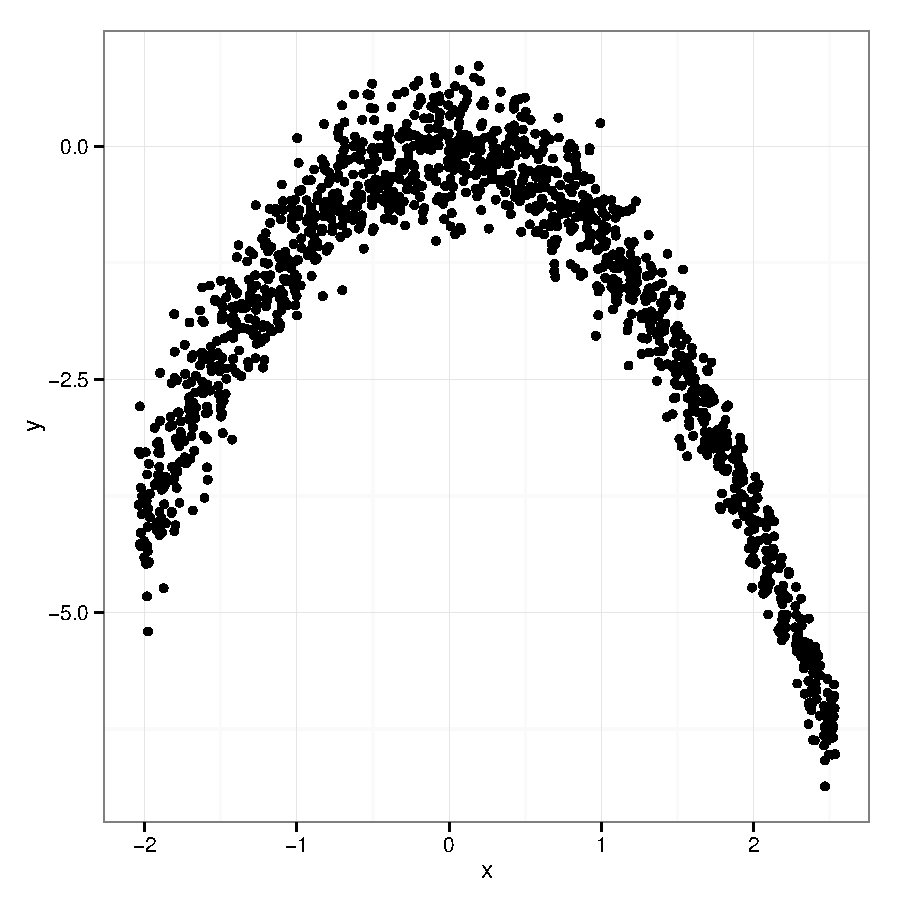
\includegraphics[width=\textwidth]{fig-cleveland1}
  \caption{\small Data}
  \label{fig:clevelandsubfig1}
\end{subfigure} \hfill\hfill
\begin{subfigure}[b]{.45\textwidth}
  \centering
  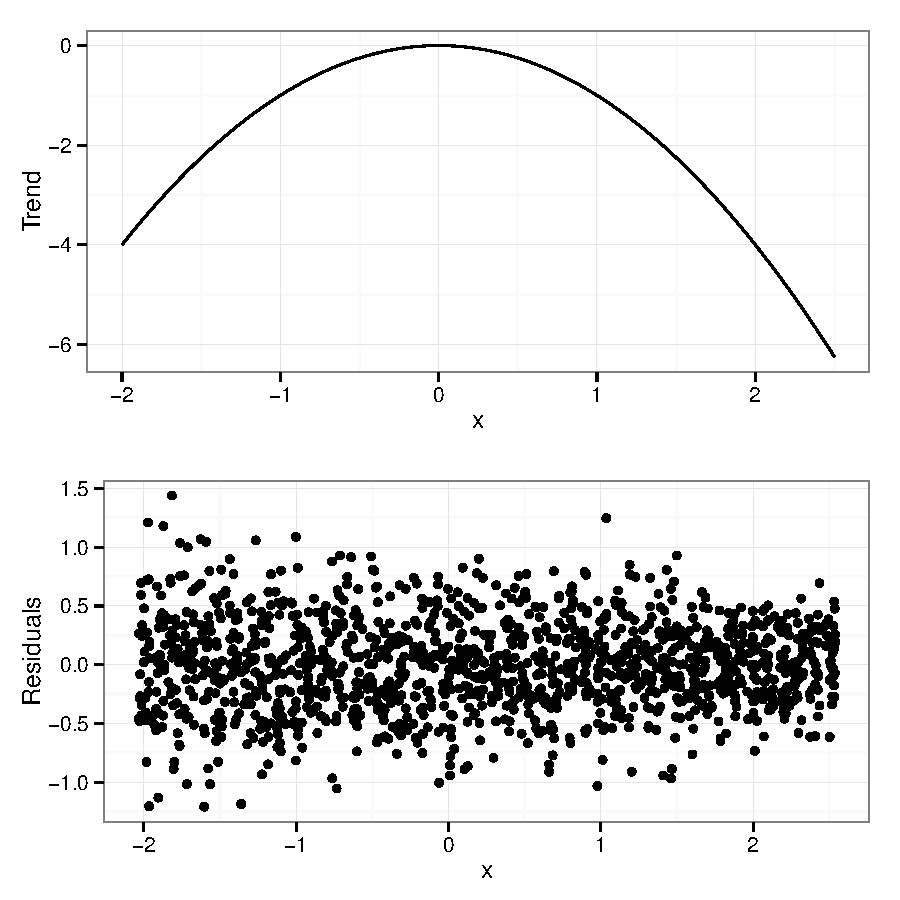
\includegraphics[width=\textwidth]{fig-cleveland2}
  \caption{\small Trend and Residuals}
  \label{fig:clevelandsubfig2}
\end{subfigure} \hfill
\caption[Changing variability and nonlinear trend lines]{Describe the conditional variability of the points along the $x$ axis in (a). Is your description consistent with the residual plot in (b)?}
\label{fig:cleveland-figure}
\end{figure}

%From a cognitive perspective, separating out the trendline and the variance creates a barrier to understanding the data in its original form; as the original graph must be mentally re-constructed.
Additionally, removing the trend requires an initial model, making any plots produced using that fit conditional on the assumptions necessary to obtain that model fit. In many situations, this may be undesireable. In particular, we typically view the data before fitting even a rudimentary model, and the sine illusion may influence even these initial modeling decisions.

\subsection{Transformation of the $X$-Axis}
As the sine illusion is driven by changes in the slope of trends between variables, we can counteract the illusion by removing these changes, transforming the $x$ axis such that the absolute value of the slope is constant and forcing the corresponding orthogonal width to represent the conditional variability.
In order to describe this transformation of the $x$ axis mathematically, 
let us assume that the relationship between variables $X$ and $Y$ is given by a  model of the form 
\[
y = f(x) + \varepsilon,
\]
where $f$ is some underlying function (either previously known or based on a model fit). Further let us assume that  $f$ is differentiable over the region of observed data.

Ideally, the correction would force all lines to appear under the same slope, i.e.~we want to find a transformation $T(x)$ of $x$, such that $f(T(x))$ is a  piece-wise linear function, where each piece has the same absolute slope. This transformation has an effect similar to ``banking to 45$^\circ$" in a piecewise manner. 

Let $a$ and $b$ be the minimum and maximum of the $x$-range under consideration. Then for any value $x \in (a,b)$ the following transformation results in a function with constant absolute slope:
\begin{equation}\label{eqn.xtrans}
(f \circ T)(x) = a + (b-a)\left(\int_{a}^x |f^\prime(z)| dz\right)/\left(\int_{a}^{b}|f^\prime(z)| dz\right),
\end{equation}

\subsubsection{Derivation of the X Transformation}\label{app.xtrans}
As the slope is determined by the aspect ratio, we are free to choose it and w.l.o.g. we get for each piece $T_i$: 
\[
f(T_i(x)) = \pm a x + b_i.
\]
This means that $T_i$ is essentially an inverse of function $f$, with each piece defined by the   intervals on which the inverse of $f$ exists: let $\left\{x_0 = \min(x), x_1, ..., x_{K-1}, x_K = \max(x) \right\}$ be the set of values with local extrema enhanced by the boundaries of the $x$-range, i.e.  $f^\prime(x_i) = 0$ for  $i = 1, ... , K-1$ and $f^\prime(x) \neq 0$ for any other values of $x$. 
Then each interval of the form $(x_{i-1}, x_i)$ defines one piece $T_i$ of the transformation function $T(x)$. We will define $T_i$ now as a combination of a linear scaling function and the inverse of $f$, which we know exists for interval $(x_{i-1}, x_i)$.

Let function $s = \s{[a,b]}{[c,d]}$ be the linear scaling function that maps  the interval $(a,b)$ linearly to the interval $(c,d)$. This function is formally defined as
\[
s(x) = \s{[a,b]}{[c,d]} (x) = (x-a)/(b-a) \cdot (d-c) + c \text{ for all } x \in (a,b).
\]
Note that the slope of function $s$ is given as
\[
s^\prime(x) = (d-c)/(b-a).
\]
%
Two scaling functions can be evaluated one after the other, only if the image (i.e. $y$-range) of the first coincides with the domain (i.e. $x$-range) of the second. This consecutive execution results in another linear scaling: 
\[
\s{[e,f]}{[c,d]}  \left(  \s{[a,b]}{[e,f]}(x) \right) = \s{[a,b]}{[c,d]} (x)
\]


In our situation let the scaling function $s$ be given as:
\[
\s{[c,d]}{f([x_{i-1}, x_i])}(x) = f(x_{i-1}) + (x-c)/(d-c) \cdot (f(x_{i}) - f(x_{i-1}))),
\]
where $f([x_{i-1}, x_i])$ is defined as the interval given by $(\min(f(x_{i-1}), f(x_i)), \max(f(x_{i-1}), f(x_i)))$.
Note that $s$ has either a positive or negative slope depending on whether $f(x_{i-1})$ is smaller or larger than $f(x_i)$, respectively.

Then the transformation in the $x$-axis, $T(x)$ is defined piecewise as a combination of $T_i$, where each $T_i$ is given as:
\begin{eqnarray}\label{eq.x.transformation}
T_i(x) &=& f^{-1}\left( \s{[c_i,d_i]}{f([x_{i-1}, x_i])}(x) \right). 
\end{eqnarray}
%
Using this definition for the transformation makes $f(T(x))$ a piece-wise linear function with parameters $c_i$ and $d_i$, i.e. for $x \in (c_i,d_i)$ we have
\[
f(T(x)) = f (f^{-1}(\s{[c_i,d_i]}{f([x_{i-1}, x_i])}(x))) = \s{[c_i,d_i]}{f([x_{i-1}, x_i])}(x).
\]
Correspondingly, the slope of $f(T_i(x))$ is $(f(x_{i}) - f(x_{i-1})))/(d_i-c_i)$.
In order to make the slope the same on all pieces $T_i$ of $T$, we need to define $c_i$ and $d_i$ with respect to the function values on the interval $(x_{i-1}, x_i)$. There are various options, depending on how closely the $x$-range of $T$ should reflect the original range:
for $[c_i, d_i] = \range {f([x_{i-1}, x_i])}$ the new $x$-range is the range of $f$ on $(x_{i-1}, x_i)$, but with the advantage that the scaling function simplifies to the identity or a simple shift.

In order to preserve the original $x$-range, we need to invest into a bit more work for the scaling. With an identity scaling, each $T_i$ maps from the range of $f$ on $(x_{i-1}, x_i)$ to the same range. Overall we can therefore set up the function $T$ to map from the interval given by the sum of the function's `ups' and `downs', i.e.
$(0, \sum_{i=0}^K |f(x_i) - f(x_{i-1})|)$, to the range of $f$ on $(x_0, x_K)$.  This ensures that all pieces $f(T_i)$ have the same slope (of $|1|$).We can then use another - global - linear scaling function to map from the range of $x$, i.e. interval $(x_0, x_K)$ to $(0, \sum_{i=0}^K |f(x_i) - f(x_{i-1})|)$, yielding a transformation function $T$ of

\[
T (x) =  (f^{-1} \circ \s{[c_i,d_i]}{f([x_{i-1}, x_i])} \circ \s{(x_0, x_K)}{(0, \sum_{i=0}^K |f(x_i) - f(x_{i-1})|)}) (x),  
\]
where $c_i$ and $d_i$ are given as 
\[
c_i = \sum_{j=0}^{i-1} |f(x_j) - f(x_{j-1})| \text{ and } d_i = \sum_{j=0}^{i} |f(x_j) - f(x_{j-1})|.
\]
We can write the difference $|f(x_j) - f(x_{j-1})|$ as $\int_{x_{j-1}}^{x_j} |f^\prime(z)|dz$. This shows equation (\ref{eqn.xtrans}).

\subsubsection{Weighting the X Transformation}
 As the sine illusion depends on changing slope in the overall trend,  re-parametrizing the $x$-axis in terms of the slope will make the data  appear under a  constant slope, thereby removing the effect of the illusion, while the transformed $x$-axis is changed from a linear representation of the $x$ values to a `warped' axis that continuously changes the scale of $x$ to compensate for the changes in the slope.
 To emphasize this change in scale along the $x$ axis,  dots are drawn at  the bottom of the chart  to show the transformation's effect on equally spaced points along the $x$-axis.   

Results from this transformation are demonstrated in Figure \ref{fig:xtrans1}.
 



\begin{figure}[h!tbp]\centering
\begin{subfigure}[b]{.45\textwidth}\centering 
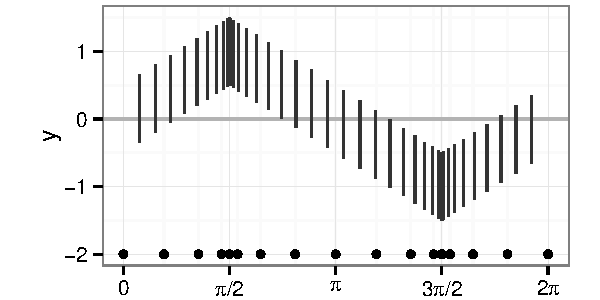
\includegraphics[keepaspectratio=TRUE,width=\textwidth]{fig-xtransform1}
\caption[$X$ axis transformation]{$X$ axis transformation based on eqn.~(\ref{eqn.xtrans}), corresponding to weighting of $w=0$.}
\label{fig:xtrans1}
\end{subfigure} \hfill\hfill
\begin{subfigure}[b]{.45\textwidth}\centering
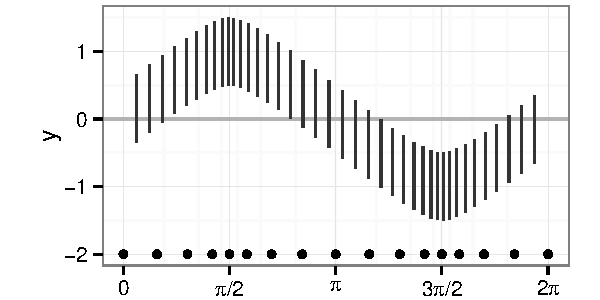
\includegraphics[keepaspectratio=TRUE,width=\textwidth]{fig-xtransform2} 
\caption[Weighted transformation]{Weighted Transformation, $w=1/2$ (based on eqn.~(\ref{eqn.xtrans.weighted}))}
\label{fig:xtrans2}
\end{subfigure}

\begin{subfigure}[b]{.45\textwidth}\centering 
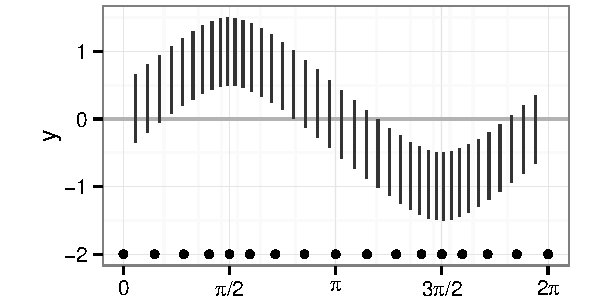
\includegraphics[keepaspectratio=TRUE,width=\textwidth]{fig-xtransform3}
\caption[Weighted transformation]{Weighted Transformation, $w=1/3$}
\label{fig:xtrans3}
\end{subfigure} \hfill
\begin{subfigure}[b]{.45\textwidth}\centering
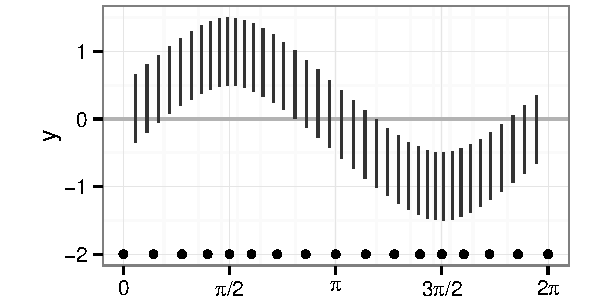
\includegraphics[keepaspectratio=TRUE,width=\textwidth]{fig-xtransform4}
\caption[Weighted transformation]{Weighted Transformation, $w=1/4$}
\label{fig:xtrans4}
\end{subfigure}
\caption[X axis transformations]{Examples of $X$ axis transformations in the sine curve.  Dots at the bottom of the graph show the transformation's effect on equally spaced points along the $x$-axis. Different amounts of weighting $w$ correspond to differently strong corrections. In (a),   $x$-spacing of the lines changes the extant width such that the absolute value of the slope is uniform across the whole range of the $x$ axis resulting in the largest amount of correction.  (b) - (d) reduce the correction in (a) towards successively more uniform spacings in $x$ while still breaking the effects of the illusion.}
\label{fig:xtrans}
\end{figure}
While the transformation in equation (\ref{eqn.xtrans}) effectively removes the appearance of changing line lengths, we can see in practice that the illusion can be broken by a much less severe transformation of the $x$ axis. 
For that we introduce a shrinkage factor $w \in (0,1)$ that allows a weighted approach in counteracting the illusion as: 
%
\begin{equation}\label{eqn.xtrans.weighted}
(f \circ T_w)(x) = (1-w) \cdot x + w \cdot (f \circ T)(x)
\end{equation}
%
Note that for $w=1$ the $x$-transformation is completely warped, while smaller values of $w$ indicate a less severe adjustment against the sine illusion.  Under  weaker transformation,s the data more closely reflect the original function $f(x)$. 
Figures \ref{fig:xtrans2} - \ref{fig:xtrans4} show the effect of different shrinkage coefficients $w$. As $w$ decreases, the lines become more evenly spaced and the illusion begins to return. 

The extent  to which we can shrink the adjustment back to the original function  varies with the aspect ratio of the chart and the shape of the function. It might also be influenced by the audience's experience with the sine illusion, resulting in very subjective choices of an ``optimal weighting" for specific situations which minimizes distortion and maximizes the correspondence between inferences made from the data and inferences made using the visual display.


Note, that we only make use of the transformation $T$ in the form of $f \circ T$. This allows us to avoid an explicit calculation of the transformation $T$, which in particular  involves a computation of the inverse of $f$ leading to potentially computation-intense solutions. 
\subsubsection{X Transformation Demonstration}



In the example of the Ozone data shown in figure \ref{fig:exampleFull1}, we can base a transformation of the $x$-axis on a loess fit of ozone concentration in daily temperature. Loess is particularly convenient for this transformation, as it enforces continuity conditions including differentiability of the fitted function; software allows us to obtain fits of both the function values and their derivatives.

Figure \ref{fig:xtrans-example} shows the original data side-by-side with the transformed $x$-axis, demonstrating not only the effect of transformation of the $x$-axis, but also that the transformation is not overly misleading in this example. The granularity of the data in this example provides an implicit measure of the strength of the transformation along the $x$-axis and the transformation is also clearly evident in the labels along the $x$-axis. 
%
\begin{figure}[h!]\centering
\begin{subfigure}[b]{.48\textwidth}\centering
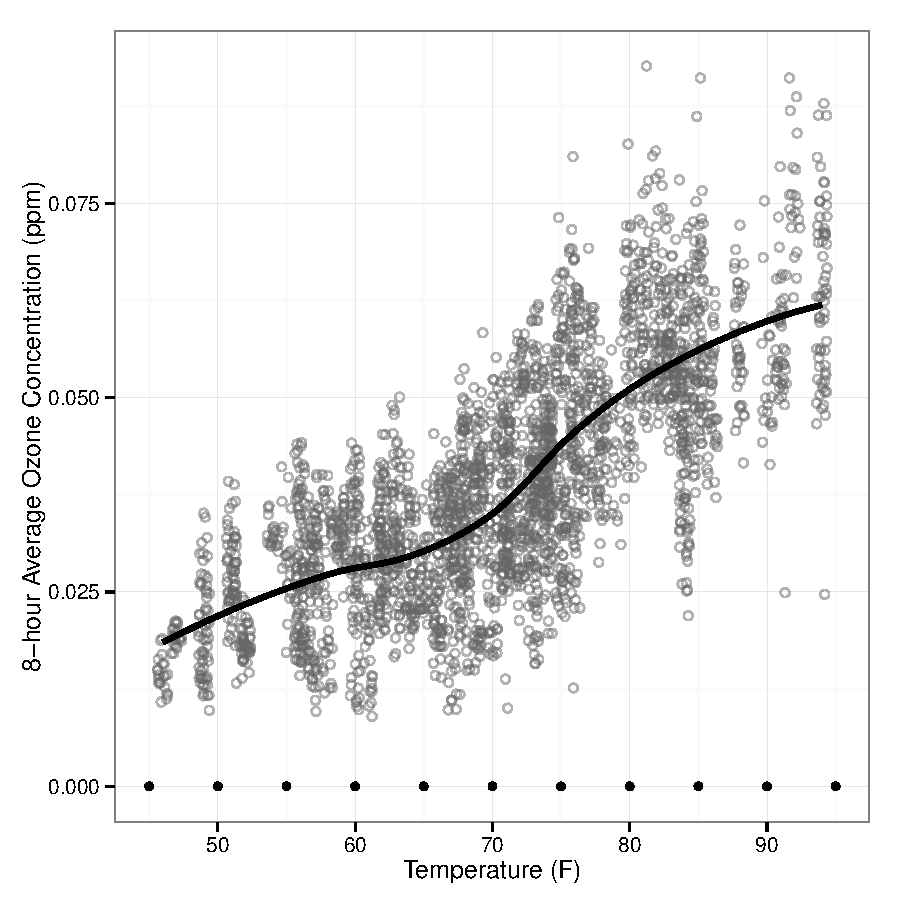
\includegraphics[keepaspectratio=TRUE,width=\textwidth]{fig-xtrans-example1}
\caption{Original Data}\label{fig:xtrans-example-original}
\end{subfigure}
\begin{subfigure}[b]{.48\textwidth}\centering
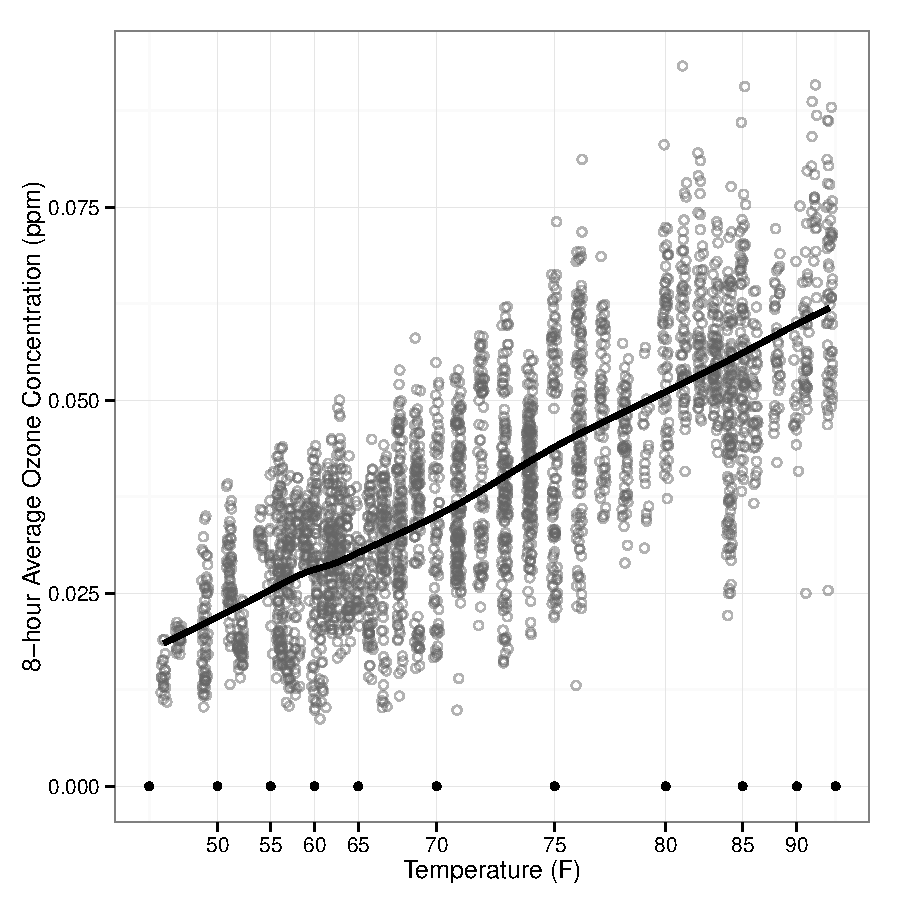
\includegraphics[keepaspectratio=TRUE,width=\textwidth]{fig-xtrans-example2}
\caption{Transformed $X$ Axis}\label{fig:xtrans-example-trans}
\end{subfigure}
\caption[Original data and data after X transformation]{Original data and data after $x$-transformation. The increasing variance is easier to see when $x$ has been transformed, because the slope is now uniform.\label{fig:xtrans-example}}
\end{figure}


\subsection{Transformation in $Y$}
Understanding the geometry of the sine illusion leads to another approach to counteracting  the conflict between the orthogonal width and the vertical length of the segment. 



Let again the function $f$ describe the general relationship between variables $X$ and $Y$. 


As sketched out in figure~\ref{fig:GeneralCorrection} we want to first find the orthogonal (extant) width in a point $(x_0, f(x_o))$ on the graph, which corresponds to the  perceived width, and then correct the vertical width accordingly to match with the audience's expectation.

\begin{figure}
\centering
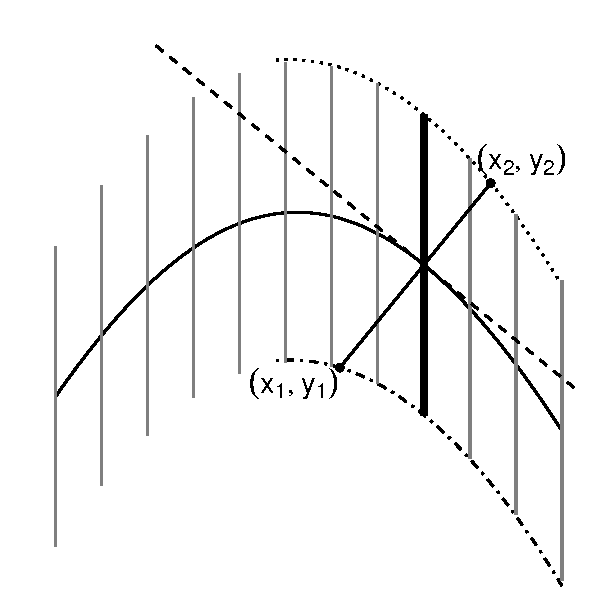
\includegraphics[keepaspectratio=TRUE,width=.33\textwidth]{fig-generalcorrectioncartoon3}
\caption[General correction approach]{ General correction approach. This approach may require numerical optimization to obtain exact solutions for $(x_1, y_1)$ and $(x_2, y_2)$.}\label{fig:GeneralCorrection}
\end{figure}

The orthogonal width (see sketch in figure~\ref{fig:GeneralCorrection}) is given as the line segment between endpoints $(x_1, f_1(x_1))$ and $(x_2, f_2(x_2))$, where $f_1$ and $f_2$ denote the vertical shifts of function $f$ by $-\ell/2$ and $\ell/2$, respectively, where $\ell$ is defined as the overall line length, $\ell > 0, \ell \in \xR$.
These endpoints are determined as the intersection of the line  orthogonal to the tangent line in $(x, f(x))$ and the graphs resulting from the vertical shifts of $f$.

The function describing the orthogonal line through $(x_o, f(x_o))$ is given in point-vector form as 
\[
{x_o \choose f(x_o)} + \lambda {f^\prime(x_o) \choose 1}, 
\]
for any real-valued $\lambda$.
The advantage of using point vector form is that it allows us to solve for parameter $\lambda$ easily, which gives us easy access to the extant (half-)widths,  as: 
\begin{equation}\label{eqn.halfwidth}
|\lambda| \sqrt{1 + f^\prime(x_o)^2}.
\end{equation}
Eqn. (\ref{eqn.halfwidth}) describes the quantity that we perceive rather than the quantity that we want to display ($\ell/2$), which leads us to a general expression of the correction factor as
\begin{eqnarray*}
 \ell/2 \cdot \left(|\lambda| \sqrt{1 + f^\prime(x_o)^2}\right)^{-1}.
\end{eqnarray*}
Note that this yields in general two solutions: one for positive, one for negative values of $\lambda$ corresponding to upper and lower (half-)extant width.

In order to get  actual numeric values for $\lambda$, we need to find end points of the extant line width as solutions of intersecting the orthogonal line and  the graphs of $f_1$ and $f_2$. We find these end points  as solutions in $x$ and $\lambda$ of the system of equations:
\begin{eqnarray}\label{eqn.general}
 x - x_o &=& \lambda f^\prime(x_o)\\ \label{eqn.general.2}
 f(x) - f(x_o) &=& -\lambda \pm \ell/2
\end{eqnarray}


Note that  the above system of equations involves function values $f(x)$, which implies that solving this system  requires numerical optimization for any but the most simple functions $f$.

In the following two sections we make use of Taylor approximations of first and second order to find approximate solutions to end points as sketched out in figure \ref{fig:linear.quadratic}.





\begin{figure}[h!]\centering
\begin{subfigure}[t]{0.4\textwidth}\centering
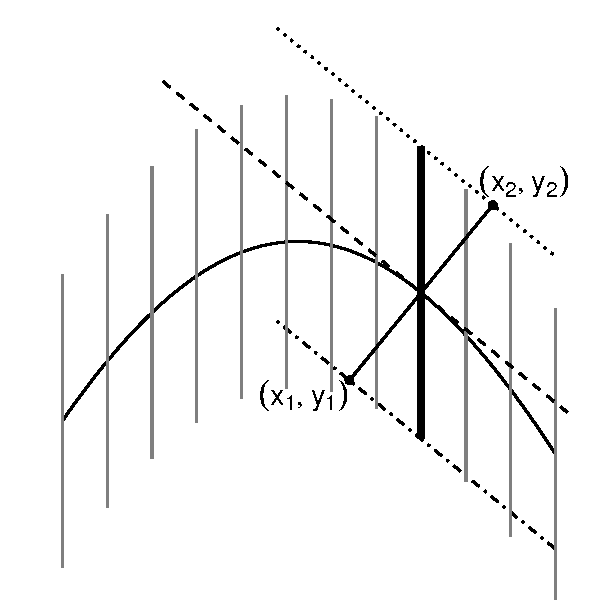
\includegraphics[keepaspectratio=TRUE,width=0.9\textwidth]{fig-generalcorrectioncartoon2}
\caption{Linear Approximation}\label{fig:linear-GeneralCorrection}
\end{subfigure}
\begin{subfigure}[t]{0.4\textwidth}\centering
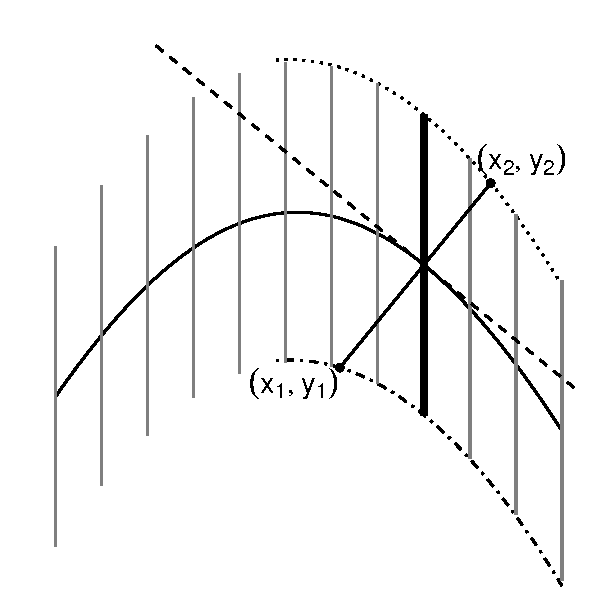
\includegraphics[keepaspectratio=TRUE,width=0.9\textwidth]{fig-generalcorrectioncartoon3}
\caption{Quadratic Approximation}\label{fig:quadratic-GeneralCorrection}
\end{subfigure}
\caption[Methods based on Approximations to f(x)]{(a) uses a first-order Taylor series approximation to $f(x)$ and (b) uses a second-order Taylor series approximation to $f(x)$. The intersection of the function $f(x) \pm \ell/2$ and the orthogonal line,  $(x_1, y_1), (x_2, y_2)$ must be obtained to determine the necessary correction factor.}\label{fig:linear.quadratic} 
\end{figure}

\subsubsection{Linear Approximation to $f(x)$}\hfill\newline
For the linear approximation we make use of $f(x) \approx f(x_0) + (x - x_0) f^\prime(x_0)$, which together with  equations~\ref{eqn.general} and \ref{eqn.general.2} yields a correction factor in $x_0$ of
\[
\ell_{\text{new}}(x_0) = \ell_{\text{old}} \sqrt{1 +  f^\prime(x_0)^2}.
\]

Note that the linear method gives the same result as a varying slope extension from a trigonometric approach  suggested by \citet{schonlau:2003} and used in \citet{marie:2013}

A second-order Taylor polynomial approximation to $f(x)$ additionally accounts for the asymmetry in the extant widths on either side of the center trendline.

\subsubsection{Quadratic Approximation to $f(x)$}\hfill\newline
Using the approximation $f(x) \approx f(x_0) + f^\prime(x_0)(x-x_0) + 1/2 f^{\prime\prime}(x_0)(x-x_0)^2$, the system of equations~\ref{eqn.general} and~\ref{eqn.general.2}  simplifies to the following  quadratic equation in $\lambda$:
\begin{eqnarray*}
f^{\prime\prime}(x_0)  f^\prime(x_0)^2 \lambda^2  + 2(f^\prime(x_0)^2 + 1) \lambda  \pm \ell = 0,
\end{eqnarray*}
which leads us to corrections for the half lengths as:
\begin{eqnarray}\label{eqn.q1}
\ell_{\text{new}_1}(x_0) &=& 1 /2 \cdot  \left(v + \sqrt{ v^2 +  f^{\prime\prime}(x_0) f^\prime(x_0)^2\cdot  \ell_{\text{old}}}\right) \cdot v^{-1/2} \\\label{eqn.q2}
\ell_{\text{new}_2}(x_0) &=& 1 /2 \cdot  \left(v + \sqrt{ v^2 -  f^{\prime\prime}(x_0) f^\prime(x_0)^2\cdot  \ell_{\text{old}}}\right) \cdot v^{-1/2} 
\end{eqnarray}
where $v = 1 + f^\prime(x_0)^2$.

\begin{subsubsection}{Reformulation of the quadratic approximation}\label{app.quadratic}
A quadratic equation in $\lambda$ of the form 
\begin{equation}\label{quadratic.equation}
a\lambda^2 + b\lambda + c = 0,
\end{equation}
where $a, b,$ and $c$ are real-valued parameters the solutions take on the form
\begin{eqnarray*}
\lambda_{\pm} = \frac{-b \pm \sqrt{b^2 - 4ac}}{2a}
\stackrel{*}{=} 2c\left(-b \pm \sqrt{b^2 - 4ac}\right)^{-1}.\\
^*\text{ if } b \neq \pm &\sqrt{b^2 - 4ac}\text{, i.~e. }a, c \neq 0.
\end{eqnarray*}

\paragraph{Application to quadratic approximation to $f$:}
in the example, we have the following equivalencies:
\begin{eqnarray*}
a &=& f^{\prime\prime}(x_0) f^\prime(x_0)^2 \\
b &=& 2(1 + f^\prime(x_0)^2) \hspace{.5in} > 0 \text{ for all } x \\
c &=& \pm \ell 
\end{eqnarray*}
For a valid solution for the correction factor, we have to assume that $\lambda$ is a factor that extends the original extant width (in absolute value). 

\begin{eqnarray*}
\lambda_{1/2} &=& \ell \left(v + \sqrt{ v^2 \pm  f^{\prime\prime}(x_0) f^\prime(x_0)^2\cdot \ell}\right)^{-1} 
\end{eqnarray*}
for $v = 1 + f^\prime(x_0)$. 
This gives the results as shown in equations (\ref{eqn.q1}) and (\ref{eqn.q2})
\end{subsubsection}

\begin{figure}
\begin{subfigure}[b]{.32\textwidth}\centering
\begin{knitrout}
\definecolor{shadecolor}{rgb}{0.969, 0.969, 0.969}\color{fgcolor}

{\centering 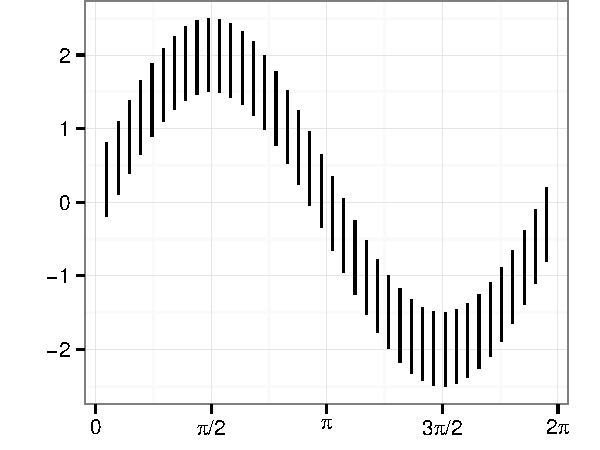
\includegraphics[width=\textwidth]{../Figure/sineIllusion/fig-UncorRresults} 

}



\end{knitrout}

\caption{Uncorrected}
\end{subfigure}
\begin{subfigure}[b]{.32\textwidth}\centering
\begin{knitrout}
\definecolor{shadecolor}{rgb}{0.969, 0.969, 0.969}\color{fgcolor}

{\centering 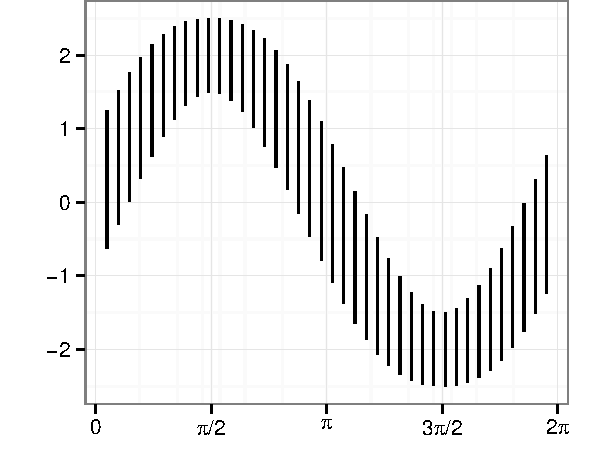
\includegraphics[width=\textwidth]{../Figure/sineIllusion/fig-LinearResults} 

}



\end{knitrout}

\caption{Linear correction}
\end{subfigure}
\begin{subfigure}[b]{.32\textwidth}\centering
\begin{knitrout}
\definecolor{shadecolor}{rgb}{0.969, 0.969, 0.969}\color{fgcolor}

{\centering 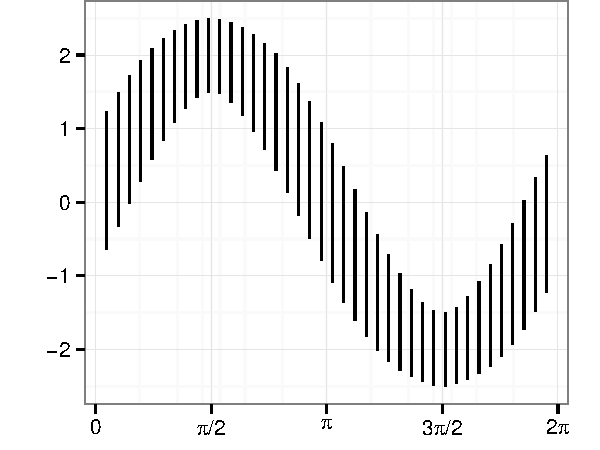
\includegraphics[width=\textwidth]{../Figure/sineIllusion/fig-CtsAdjustedResults} 

}



\end{knitrout}

\caption{Quadratic correction}
\end{subfigure}
\caption[Quadratic Approximation]{
In the quadratic approximation top and bottom segments of the vertical lines are adjusted separately.}
\label{fig:GeneralQuadraticCorrection} 
\end{figure}

Adjusting the top and bottom segments of the vertical lines separately so that the extant width is constant breaks the illusion, but slightly distorts the sinusoidal shape of the peaks.

Figure~\ref{fig:GeneralQuadraticCorrection} shows the correction factor based on a quadratic approximation compared to the untransformed data. 
Unlike the linear solution, the half-segments here are not necessarily of the same length, and thus there are separate correction factors for each half-segment. 



\subsubsection{Mathematical Properties of the Y Transformation}
The quadratic correction breaks whenever the expression in the square root of eqn.~(\ref{eqn.q1}) becomes negative, i.e.~whenever $v^2 \pm \ell\cdot f^{\prime\prime}(x)\cdot f^\prime(x)^2 < 0$.
This happens for  combinations of large values of $\ell$, which signify a large vertical extent, or large conditional variability $E[Y|X]$, and simultaneous large changes in the slope of the main trend, i.e.~large values of the curvature $f^{\prime\prime}(x)$. In the linear approximation of $f$ the same situation leads to a massive overcorrection of the vertical lines, changing the shape of the `corrected' function beyond recognition.

Similar to the correction of the $x$-axis,  we can use a weighted approach to find a balance between counteracting the illusion and representating the  original data:
\begin{equation}\label{eqn.ytrans.weighted}
\ell_{new_w}(x) = (1-w) \cdot \ell_{old} + w \cdot \ell_{new}(x)
\end{equation}

\section{Transformations in Practice -- a User Study}

In order to more fully understand the sine illusion and test the proposed corrections, we created an applet to allow users to investigate the illusion's prominence with respect to its parameters. Users can examine the sine illusion by changing line length, the function's amplitude, and compare corrections in $x$-axis and $y$-values to uncorrected data.  All corrections proposed in this paper are  implemented in the applet located at \url{http://glimmer.rstudio.com/srvanderplas/SineIllusion/}.

We employed a second applet to collect data on users' preferences on the amount of correction used, i.e.~we are interested in identifying a range of `optimal weights' in each of the corrections. This applet presents users with a graph that is the result of a correction in $x$ or $y$ with a randomly selected starting weight value. Users are asked to adjust the graph until the illusion  (a) is no longer apparent (adjustment of weights from the bottom) or (b) becomes visible (adjustments of weights from the top).

Both applets are implemented in {\tt shiny} \citep{shiny}. 

The graphs in the data-collection applet are adjusted using a plus/minus button to either increase or decrease the amount of correction used. Underlying this adjustment is the value of the weight $w$ as defined in eqns.~(\ref{eqn.xtrans.weighted}) and~(\ref{eqn.ytrans.weighted}). The numerical value of $w$ was hidden from the user to prevent anchoring to a specific numerical value.

A low  initial weight ($w_0$ close to 0) indicates that the amount of correction is low and the response from a trial like this will give us an idea of the minimal amount of weight necessary to break the illusion, while a high initial weight ($w_0$ close to 1) indicates that the data is fully corrected. We asked participants to change the amount of adjustment until the lines appear to be the same length assumes that the correction is overcorrecting in practice, and a response from this type of trial gives us an upper boundary for the amount of weighting preferred. Generally, responses from the two different types of trials do not result in the same threshold weight, but rather lead to a range of acceptable weights.

It is of additional interest to determine whether and how much these optimal weights are subject-specific or population-based, whether they depend on the initial weight, and how much within-subject variability we find compared to between-subject variability. 

\begin{figure}\centering
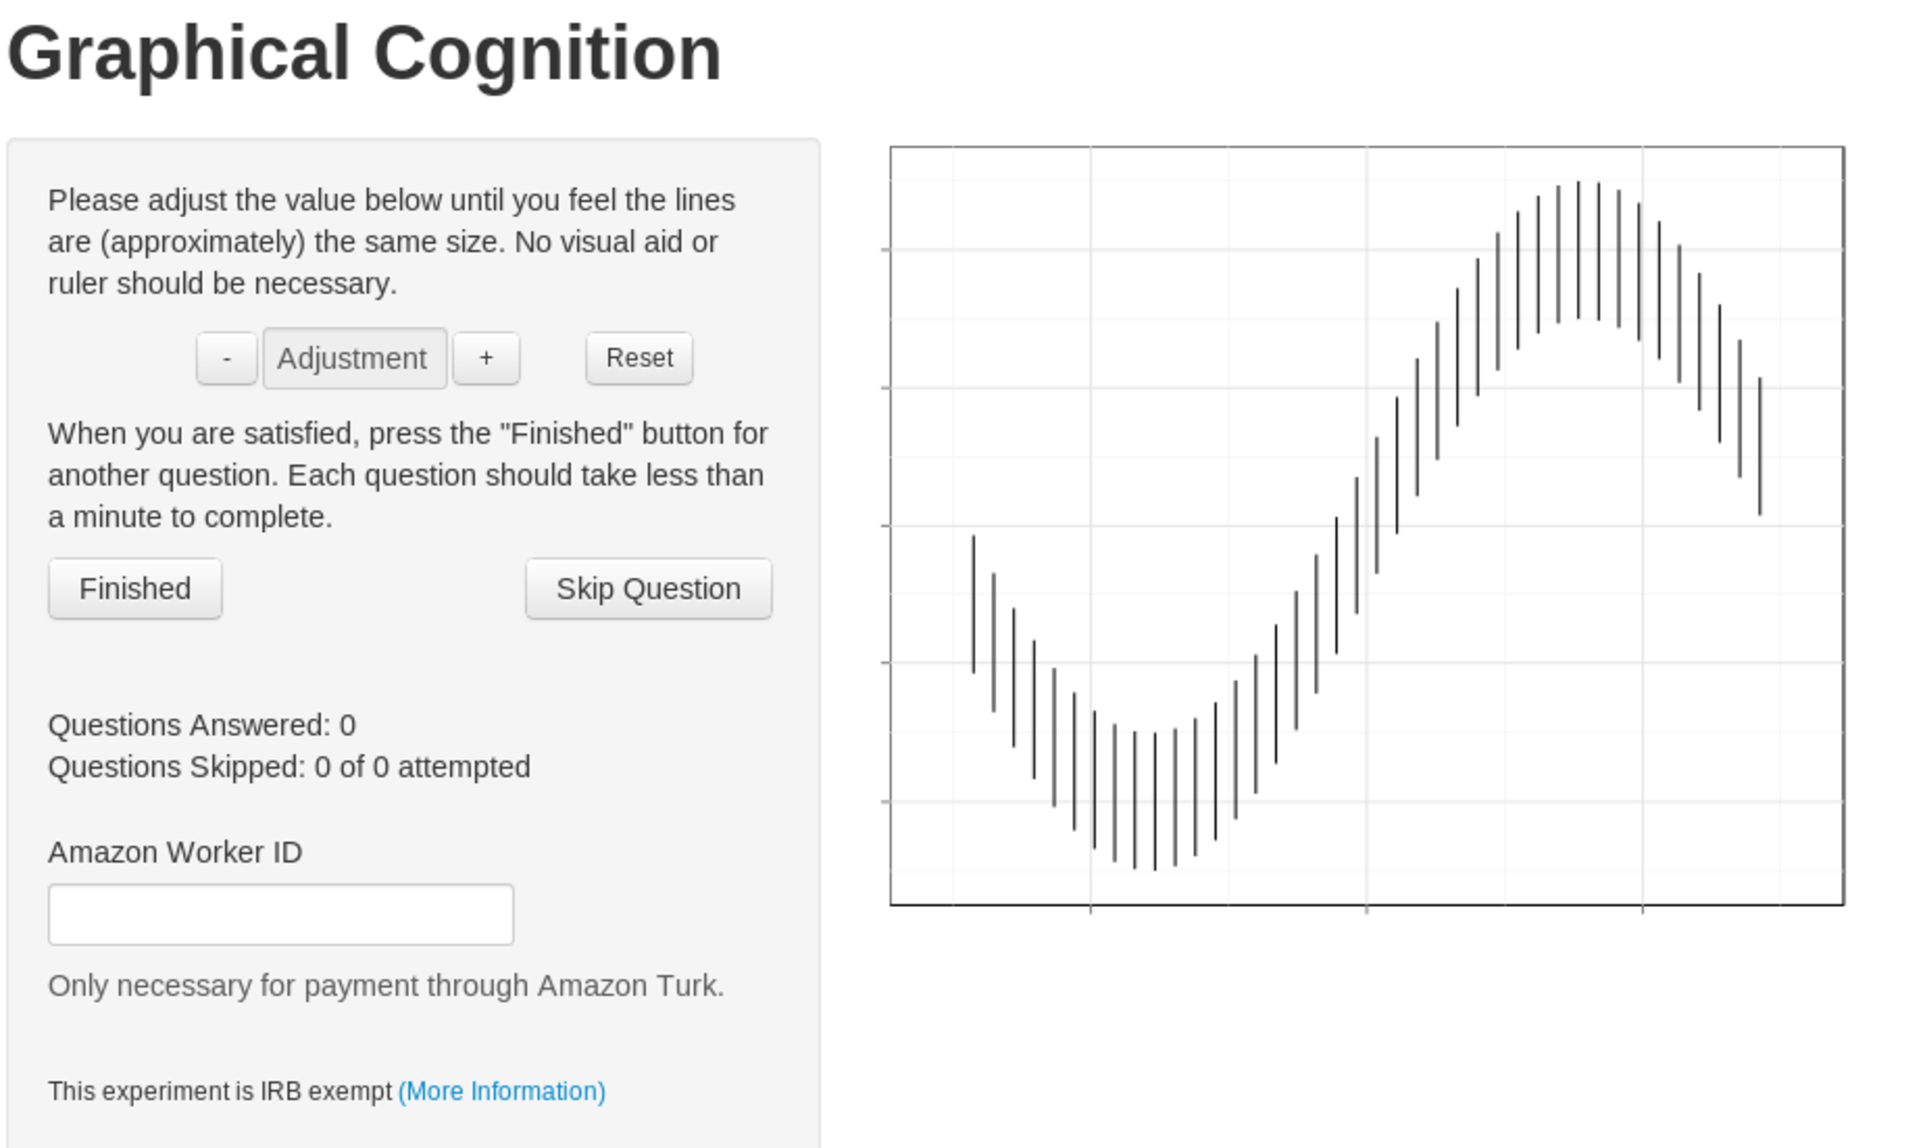
\includegraphics[width=.92\textwidth]{shiny}
\caption[Screenshot of Data Collection Website]{\label{fig:shiny.app} Screenshot of the shiny application used to collect information of observers' preference with respect to an optimal correction for the illusion under each of the  transformations discussed in the previous section. }
\end{figure}

Figure~\ref{fig:shiny.app} shows a screenshot of the applet used to collect user data. This applet is  available online at \url{http://glimmer.rstudio.com/srvanderplas/SineIllusionShiny/}. 
Line length and function are controlled in this app, and we used the linear transformation for adjusting $y$ values; the transformation does not break under any combination of parameters tested in this experiment. 


\noindent
We deployed the applet to participants recruited online, collecting their responses and other metadata. The results of the analysis suggest that the correction factors in $X$ and $Y$ are both preferrable to uncorrected data, but that a full correction is not necessary to break the illusion.




\subsection{Study Design}
The study aims to determine the range of ``optimal'' transformation weights for each transformation type. Psychophysics methodology typically approaches threshold estimation by using the method of adjustment \citep{goldstein}, where  stimuli are provided showing states both above and below the hypothesized optimal value and  participants adjust the stimuli until the stated goal is met (in this case, until the lines appear to have equal length). It is expected that there will be a difference in user-reported values from below and from above, and these values are typically averaged to produce a single threshold value. Beyond averaging these values, we use a mixed model to compare user responses for different starting points in a more continuous fashion, incorporating some of the advantages of the method of constant stimuli to more robustly estimate the range of optimal transformation weights. For a review of general psychophysics methodology, the method of adjustment, and the method of constant stimuli, see \citet{goldstein}.

The study is set up as a fractional factorial design of correction type ($x$ or $y$ correction) and starting weight $w_0$. Each participant is asked to evaluate a total of twelve situations, six of each correction type.
Starting weights were chosen as follows: each user was given a trial of each type starting at 0 and 1. The remaining four trials of each type had starting weights chosen with equal probability from $0.25$ to $0.75$ 
(see figure~\ref{fig:weightdist}). 
We decided to  have a higher coverage density for starting weights around 0.6 after a pilot study indicated a preference for that value. Using a distribution with a wide coverage allows us to more fully explore the space of plausible weights $w$ while focusing on the $(0,1)$ interval and enabling precise estimation of the optimal weight in the region indicated by the pilot study.

\begin{figure}\centering
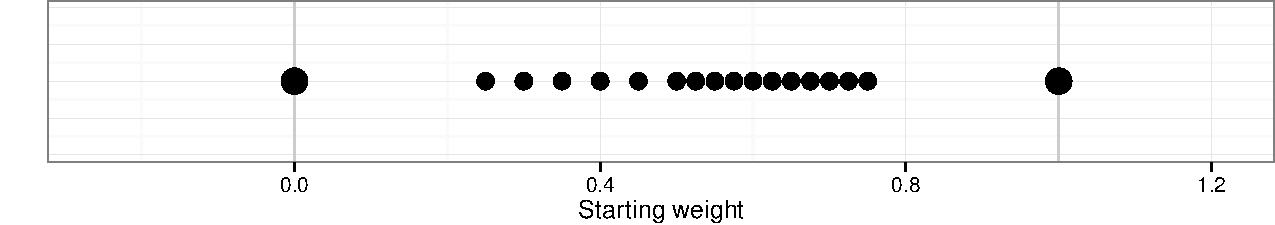
\includegraphics[keepaspectratio=TRUE,width=0.8\textwidth]{fig-study-weight-dist}
\caption[Overview of possible starting weights]{Overview of possible starting weights. Weight values are discrete, but staggered so as to provide fine-grained adjustments around 0.6 and more coarse discriminatory information toward the outside.}\label{fig:weightdist}
\end{figure}

A trial begins with the presentation of a graph at the chosen starting weight $w_0$. Participants adjust the graph using increment and decrement buttons. A trial ends with the participant clicking the `submit' button, at which point the weight for the final adjustment is recorded. This provides a clear starting value and ending value, allowing us to assess the range of optimal values for each participant. In addition to starting weight, correction type, and anonymized user-specific data (partial IP address, hashed IP address, and hashed browser characteristics), each incremental user chosen weight is recorded with a corresponding timestamp. The user-specific browser data is sufficient to provide a `fingerprint' to distinguish and recognize individual users (or rather their computer settings) in an anonymous fashion. 

Each participant is provided with two initial ``training'' trials in which the  graph of the underlying mean function is superimposed on the line segments to give participants some idea of the  function the lines represent. This approach was taken to reduce  incidences of extremely high  correction values under the $X$ transformation, as large adjustment values do not change the impression of same line length, but the resulting function bears little resemblance to a sine function, see figure~\ref{fig:overtransform} for examples of overcorrection.







\begin{figure}\centering
\includegraphics[keepaspectratio=TRUE,width=.8\textwidth]{fig-overcorrectlimits}
\caption[ Overcorrected transformations excluded from the analysis]{Transformation weights outside of the intervals $[\ensuremath{-2.5}, 3.5]$ for $y$ and $[\ensuremath{-2}, 2]$ for $x$  produce figures which do not maintain the underlying function shape (in $x$) or which are composed of extremely uneven length lines (in $y$). Trials with final results that were more extreme than these examples were excluded from the analysis.}
\label{fig:overtransform}
\end{figure}

\subsection{Results}

Participants were recruited from Amazon Mechanical Turk and the \href{http://reddit.com/r/SampleSize}{reddit} community.

As this study was conducted outside a laboratory setting, we can not gauge a participant's willingness to follow the guidelines and put in their best effort. This, besides potential technical issues (server outage, speed of response) make a careful selection of data going into the analysis unavoidable. The following exclusion criteria were used:
\begin{itemize}
\item Participants did not interact with the applet: we required participants to use the adjustment at least once in order to include data for this trial (592 trials removed).
\item Participants finished fewer than four trials: while participants were asked to complete twelve trials, some did not finish all of those. In order to stabilize predictions of random effects, participants' data were excluded if there were fewer than four trials (78 out of a total of 203 participants).
\item Out-of-bounds results: weights leading to severely over- or undercorrected results were excluded from the analysis. 
For trials to adjust $Y$-values, weights outside of [\ensuremath{-2.5}, 3.5]  show dramatically unequal line lengths; weights from $X$-transformations outside the range of [\ensuremath{-2}, 2] do not preserve the underlying function shape and concavity. 
Figure~\ref{fig:overtransform} shows results at the threshold of acceptability. Only more severely distorted results were excluded from the analysis (12 of the $X$ and 5 of the $Y$ trials out of 1227 trials remaining after application of other criteria).
\end{itemize}


The following analysis is based on the cleaned data, consisting of 125 participants with 1210 valid trial results. The psychophysics model shown in figure \ref{fig:psycho} is based on  weighted averages (by adjustment type) of all trials with starting weights $w_0 = 0$ and 1.


\begin{figure}\centering
\begin{knitrout}
\definecolor{shadecolor}{rgb}{0.969, 0.969, 0.969}\color{fgcolor}

{\centering \includegraphics[width=.5\textwidth]{../Figure/sineIllusion/fig-meanDists} 

}



\end{knitrout}

\caption[Results from psychophysics analysis]{Estimated density of participant-level means using the standard psychophysics method of limits analysis. The overall means are both near 0.4, however, there is quite a bit of user-level variability.\label{fig:psycho}}
\end{figure}




According to this analysis, the optimum transformation value for $x$ is 0.35, and the optimum transformation value for $y$ is 0.45. Figure \ref{fig:psycho} shows the estimates and 95\% Wald intervals for the mean, as well as estimated density of participant-level responses. 

While these results suggest that the transformation is useful and that complete transformation is not necessary, we can get more precise bounds on the range of acceptable transformation weights using a linear model that can incorporate starting points other than 0 and 1, and at the same time allow for user-specific variability.

In order to account for user-level variability, we fit a random effects model for the adjusted weight value as a function of  starting weight and trial type, with a random intercept for each participant. 

Let $W_{ij}$ denote the final adjustment to weight by participant $i$, $ 1 \le i \le 125$ , on trial $j$, $1 \le j \le n_i$. 
We model the final weight $W_{ij}$ as a function of the correction type $T(i,j)$  (where $T(i,j) \in  \{X, Y\}$), and starting weight $X_{ij}$, with a random intercept for participant to account for subject-specific ability: 
\begin{align}\label{model1}
W_{ij} &= \alpha_{T(i,j)} + \beta X_{ij} + \gamma_{i, T(i,j)} + \epsilon_{ij}\\
& \gamma_{iX} \stackrel{\text{ i.i.d.}}{\sim} N(0, \eta_X^2) , \ \gamma_{iY} \stackrel{\text{ i.i.d.}}{\sim} N(0, \eta_Y^2) ,\notag  \\
& \epsilon_{ij} \stackrel{\text{ i.i.d.}}{\sim} N(0, \sigma^2)  \text{ and } \text{Cov}(\gamma, \epsilon) = 0\notag 
\end{align}
 $\alpha_{T(i,j)}$ is either $\alpha_X$ or $\alpha_Y$, describing the lower threshold of the acceptable range for each of the types of correction, while $\alpha_X+\beta$ and $\alpha_Y + \beta$ describe the upper thresholds for the respective correction.

We can therefore interpret $\beta$ as the length of the interval of plausible weights. Additionally, this allows the interpretation of the quantity $(\alpha_* + \beta/2)$ as equivalent to the estimate of the optimal weight based on the psychophysics methodology.

\noindent
The fitted model parameters are shown in tables \ref{fixedeffectsresults} and \ref{randomeffectsresults}. 



\begin{table}[htbp]\centering
\begin{tabular}{cclcc}
  \hline
Transformation & Threshold &  \multicolumn{1}{c}{Parameter} & Estimate & 95\% C.I. \\ 
  \hline
X & Lower & $\alpha_X$ & 0.097 & (0.045, 0.150) \\ 
   & Upper& $\alpha_X + \beta$  & 0.625 & (0.570, 0.682) \\ 
  Y & Lower& $\alpha_Y$  & 0.143 & (0.097, 0.188) \\ 
   & Upper& $\alpha_Y + \beta$  & 0.671 & (0.626, 0.718) \\ 
   \hline
\end{tabular}
\caption[Fixed Effects]{Fixed effect estimates of model~(\ref{model1}) for the boundaries for reasonable weights. In parentheses,  95\% parametric bootstrap confidence intervals are given based on model (\ref{model1}) ($N$=1000).}\label{fixedeffectsresults}
\end{table}
\begin{table}[hbtp]\centering
\begin{tabular}{rcccc}
  \hline
Groups & Correction & Parameter & Estimate & 95\% C.I. \\ 
  \hline
  Participant & X &$\eta_X$  & 0.171 & (0.167, 0.247) \\ 
  Participant & Y &$\eta_Y$ &  0.145 & (0.107, 0.179) \\ 
  Residual &  &$\sigma$ &  0.304 & (0.290, 0.317) \\ 
   \hline
\end{tabular}
\caption[Random Effects]{Overview of random effects for model~(\ref{model1}), including 95\% confidence intervals based on parameteric boostrap results ($N$=1000).}\label{randomeffectsresults}
\end{table}

Table \ref{randomeffectsresults} gives an overview of the variance estimates. 95\% confidence intervals are, based on 1000-fold paramteric bootstrap of model~\ref{model1}. All variance components are significant and relevant; variability within a single individual's trials is about half the size of variability across  participants. 

We use parametric bootstrap to generate responses for each correction type and each participant from the model, which we use to both  create user-level densities, population-level densities, and bootstrap intervals for model parameters. 


The variability of the random effects for each trial type is similar; but the model benefits significantly from allowing separate random effects for individual's variability by correction type (0.1452 and 0.1705 for $Y$ and $X$ transformations, respectively, as opposed to 0.3044 for the overall variability). The interaction between starting weight and trial type was not significant, however, and was thus removed from the model ($p$-value = 0.901).

\begin{figure}[hbtp]
\centering
\includegraphics[keepaspectratio=TRUE, width=.85\textwidth]{fig-results-analysis1}
\caption[Results from mixed model]{Simulation results from the fitted model, facetted by correction type. Fixed effects results are shown as histograms; the red values display the results when starting from an uncorrected plot and are concentrated around $w=0.1$ for $X$ and $w=0.14$ for $Y$; the blue values represent user-chosen weights when starting from a fully corrected plot and are concentrated around $w=0.63$ for $X$ and $w=0.67$ for $Y$. Additionally, 95\% bootstrap intervals are shown as horizontal line segments above the histograms; these intervals are for the lower and upper bounds of the ``preferred weight interval" tested in the experiment. User-level density curves show the individual variability around  fixed effects $\alpha_*$ and $\alpha_*+\beta$.}\label{fig:MixedModelResults}
\end{figure}
Figure \ref{fig:MixedModelResults} gives an overview of the relationship between starting weights and  user-preferred weight values. Higher starting weights are associated with higher user-submitted values, and lower starting weights are associated with lower user-submitted values.

The ranges of optimal weights are similar under both transformations. Boundaries for the $X$ transformation are slightly lower than boundaries for $Y$. 

Bootstrap simulations for each of the coefficients suggest that the range of optimal $w$ is between 0.098 and 0.625 for $x$ and 0.142 and 0.67 for $y$, where the lower value is the estimate starting at $w=0$ and moving up, and the upper value is the estimate starting at $w=1$ and moving down. This suggests that either correction is preferrable to an uncorrected graph, and that a weighted correction is preferrable to the fully corrected graph, as neither 0 nor 1 is contained in any overall interval. In addition to showing the strength of the correction, this experiment also demonstrates the strength of the illusion itself: a correction appears more uniform than the uncorrected values, even though the corrected values are not uniform and the uncorrected values are completely uniform. 

\section{Application: US Gas Prices}
Figure~\ref{fig:gasprices} shows daily gas prices for a time frame between 1995 to 2014 as published in the Energy Information Administration's historical database of gas prices \citep{EIA}. This data includes prices for all three grades of gasoline as well as two chemical formulations which are sold in different geographic areas across the United States (for more information, see \citep{EIA-reformulated}). 


\begin{figure}[h!tbp]
\begin{knitrout}
\definecolor{shadecolor}{rgb}{0.969, 0.969, 0.969}\color{fgcolor}

{\centering \includegraphics[width=.98\textwidth]{../Figure/sineIllusion/fig-gasprices-pictures} 

}



\end{knitrout}

\caption[US Gas prices from 1995 to 2014]{US Gas prices from 1995 to 2014. Gas prices steadily increase over the time frame, with some dramatic short-term developments. Peaks and troughs seem to exhibit more variability in daily prices than times of dramatic changes. This is an effect of the sine-illusion, which hides a fairly steady increase in variance in daily gas prices over time.}\label{fig:gasprices}
\end{figure}
\begin{figure}\centering
\begin{knitrout}
\definecolor{shadecolor}{rgb}{0.969, 0.969, 0.969}\color{fgcolor}

{\centering \includegraphics[width=.7\textwidth]{../Figure/sineIllusion/fig-gaspricevariance} 

}



\end{knitrout}

\caption[Standard deviation of daily gas prices between 1995 and 2014. ]{Standard deviation of daily gas prices between 1995 and 2014. The doubling of the standard deviation over the time frame is masked in figure \ref{fig:gasprices}.\label{fig:gasvariance}}
\end{figure}
There is a clear increase in daily gas prices over time as well as several dramatic price changes. These developments mask the steady increase in variance shown in figure~\ref{fig:gasvariance}. Instead, we perceive an increase in variability in the frequent ups and downs along the overall trend. In particular, the strong decrease in gas prices at the end of 2008 seems to be associated with a low variance. This is an effect of the sine illusion, and the actual variability in Oct 2008 is higher than previous months. In order to better judge variability along the trendline we applied the two different corrections to this data. 

For either of the corrections we use a trendline fit based on smoothing splines, which provides the necessary first and second derivatives.






Figure \ref{fig:gasprices-x-correct} shows the results from the $X$ transformation applied to the gas prices. The figure on top is a fully corrected version, while the one below only uses $w=0.36$, the midpoint of the range of experimentally determined acceptable values,  for the transformation. At $w=1$, the transformation is severe, but it becomes clear that the variance between 1995 and 2000 is lower than it is between 2009 and 2014. When $w=0.36$, the transformation is much less noticable but yields a near-constant absolute slope of the fitted line.

\begin{figure}
\centering
\includegraphics[keepaspectratio=TRUE,width=.92\textwidth]{gas-x-corrected}
\caption[Gas price data, X transformation]{Gas price data corrected using the $X$ transformation with $w=1$ and with $w=0.36$. }
\label{fig:gasprices-x-correct}
\end{figure}
The minor effect of the weighted transformation on individual x-values contrasts with the effectiveness of the transformation in reducing the illusion; this is best seen in the fitted line, which is distinctly (piecewise) curved in the uncorrected data and appears to be much more piecewise linear in the corrected data, even at the reduced weighted value. 

Similar to the $X$ transformation, the $Y$ transformation highlights local fluctuation in the variability of daily gas prices much more than the untransformed data. Figure~\ref{fig:gasprices-y-correct} shows $Y$ transformations for the data. Again, we show a full transformation (top) and a transformation based on the midpoint of the previously determined acceptable region of $w=0.40$.
in the full transformation  it is clear that the variance is nearly constant between 1995 and 2000 and then begins to increase with the price of gas. When $w=0.40$, the transformation is much less noticable, and the resulting $y$-axis scale is much more similar to the uncorrected data. 

\begin{figure}[h]
\centering
\includegraphics[keepaspectratio=TRUE,width=.92\textwidth]{gas-y-corrected}
\caption[Gas price data, Y transformation]{Gas price data corrected using the $Y$ transformation with $w=1$ and with $w=0.40$. }
\label{fig:gasprices-y-correct}
\end{figure}

\section{Conclusions}
The sine illusion is a persistent and powerful illusion that is very difficult to counteract without modifying the visual stimulus directly. While systematically modifying the data is uncommon in the statistical world, this approach is not out of place in the visual arts or architecture; as far back as 400 BC the builders of the Parthenon ensured a straight appearance of the columns from afar, by widening columns at the center, thereby counteracting the effects of the Hering illusion \citep{naturalscenes,hering}. Similarly, painters often exaggerate color hues used in shadows to account for color constancy in the brain. The systematic modifications we suggest here are also comparable to chloropleth maps, which scale a region's area based on some other variable. 

We cannot counteract the illusion and represent the data visually without an intervention that is drastic enough to counteract the three-dimensional context the sine-illusion induces. The proposals in this paper for transformations in $x$ and $y$ provide the means to temporarily correct the data as a diagnostic measure, perhaps using an applet or R package for that purpose. These corrections are significant not only because of their implications for statistical graphics, but because previous attempts to resolve optical illusions using geometry have not met with success \citep{westheimer2008illusions}. These corrections are only a first step and could be improved upon; currently, the corrections break down for extreme (secant) values, but multiple iterations of the correction procedure will likely resolve some of these issues (though iteration removes the convenience of a functional form for the transformation). Similarly, the $y$ corrections proposed here extend the line lengths (or for actual data, increase the deviation from the smooth line) -- some normalization might make the necessary corrections less noticeable. 

Our primary goal is to raise awareness of the illusion and its implications for statistics; the use of plots to guide the modeling process can leave us vulnerable to overlooking changes in the variance due to the illusion. While best practice has  been to plot the residuals separately, this removes the context of the data and is not practical before there is a model. In addition, viewer attention spans may be limited if multiple graphs are presented. The proposed transformations require only a nonparametric smooth, maintain the context of the data, and are readily interpretable. 

The data for this study was collected with approval from  IRB-ID 13-257.



\chapter{VISUAL REASONING AND STATISTICAL GRAPHICS}

Paper about lineup ability and army tests of visual reasoning


\chapter{STATISTICAL GRAPHICS AND FEATURE HIERARCHY}

Paper about lineups and feature hierarchy

%-------------------------------------------------------------------------------
% % Appendix1 file from standard thesis template
\appendixtitle
\appendix
\chapter{ADDITIONAL MATERIAL}

This is now the same as any other chapter except that
all sectioning levels below the chapter level must begin
with the *-form of a sectioning command.

\section*{More stuff}

Supplemental material.


% % An example second appendix from the example thesis thesis.tex.
\chapter{STATISTICAL RESULTS}

This is now the same as any other chapter except that
all sectioning levels below the chapter level must begin
with the *-form of a sectioning command.

\section*{Supplemental Statistics}

More stuff.

%-------------------------------------------------------------------------------
\renewcommand{\bibname}{\centerline{BIBLIOGRAPHY}}
\unappendixtitle
\newpage
\phantomsection
\addcontentsline{toc}{chapter}{BIBLIOGRAPHY}
\bibliography{mybib}

%% An example bibliography from the standard thesis template
\renewcommand{\bibname}{\centerline{BIBLIOGRAPHY}}
\unappendixtitle
\interlinepenalty=300
% For no page break use thebibnopage environment
\begin{thebibliography}{99}
\addcontentsline{toc}{chapter}{BIBLIOGRAPHY}

\bibitem[Allen, B.~S.~(1984)]{allen}
Allen, B.~S. (1984). System-assigned learning strategies and CBI.
\emph{Journal of Instructional Computing Research},
\emph{1}(1), 3--18.
\filbreak

\bibitem[Bruner, J.~(1960)]{bruner}
Bruner, J. (1960). \emph{The process of education}.
New York: Random House.
\filbreak

\bibitem[Cox, S.~R.~(1974)]{cox}
Cox, S.~R. (1974). Computer-assisted instruction and student performance
in macroeconomic principles.
\emph{The Journal of Economic Education},
\emph{6}(1), 29--37.
\filbreak

\end{thebibliography}
 % Not used... stick with bibtex
\end{document}
